%% LyX 2.2.3 created this file.  For more info, see http://www.lyx.org/.
%% Do not edit unless you really know what you are doing.
\documentclass[twoside]{iuphd}
\usepackage[T1,T2A]{fontenc}
\usepackage[utf8]{inputenc}
\setcounter{secnumdepth}{3}
\setcounter{tocdepth}{3}
\usepackage{verbatim}
\usepackage{mathrsfs}
\usepackage{enumitem}
\usepackage{pdfpages}
\usepackage{amsmath}
\usepackage{amssymb}
\usepackage{graphicx}
\usepackage[all]{xy}

\makeatletter

%%%%%%%%%%%%%%%%%%%%%%%%%%%%%% LyX specific LaTeX commands.
%% A simple dot to overcome graphicx limitations
\newcommand{\lyxdot}{.}


%%%%%%%%%%%%%%%%%%%%%%%%%%%%%% Textclass specific LaTeX commands.
\newlength{\lyxlabelwidth}      % auxiliary length 

%%%%%%%%%%%%%%%%%%%%%%%%%%%%%% User specified LaTeX commands.
\usepackage[ backend=biber]{biblatex}
\addbibresource{prop.bib}
\ExecuteBibliographyOptions{sorting=none,maxbibnames=10,doi=false,isbn=false,url=false}
\DeclareUnicodeCharacter{0229}{\c{e}}
\DeclareUnicodeCharacter{00A0}{~}
\usepackage{mmap}
\usepackage{comment}
\usepackage{framed}
\usepackage[braket,qm]{qcircuit}
\usepackage{mathrsfs}
\usepackage{setspace}
\usepackage{dsfont}

\usepackage[all]{xy}
\newcommand{\xyR}[1]{\xymatrixrowsep={#1}}
\newcommand{\xyC}[1]{\xymatrixcolsep={#1}}

%\usepackage[basic]{complexity}
\newcommand{\lang}[1]{{\ensuremath{\mathsf{#1}}}}
\newcommand{\newlang}[2]{\newcommand{#1}{\lang{#2}}}
\newlang{\usat}{UNIQUE-SAT}

\newcommand{\muB}{\ensuremath{\mu^{B}}}
\newcommand{\events}{\ensuremath{\mathcal{E}}}
\newcommand{\set}[2]{\ensuremath{\left\{ {#1}\mathrel{}\middle|\mathrel{}{#2}\right\} }}
\newcommand{\gmult}{*}
\newcommand{\Fpx}[1]{\mathbb{F}_{{#1}}}
\newcommand{\Fq}{\Fpx{q}}
\newcommand{\ff}[1]{\Fpx{#1}}
\newcommand{\ffzx}[2]{\Fpx{#1}^{{#2}\;*}}
\newcommand{\ffx}[2]{\Fpx{#1}^{{#2}}}
\newcommand{\ffzd}[1]{\ffzx{#1}{d}}
\newcommand{\ffd}[1]{\ffx{#1}{d}}
\newcommand{\VVec}[1]{\vec{\bf #1}}
\newcommand{\mathReal}{\mathbb{R}}
\newcommand{\mathComplex}{\mathbb{C}}
\newcommand{\braket}[2]{\ip{#1}{#2}}
\newcommand{\todo}[1]{\textbf{TODO.~#1}}
\newcommand{\Eq}[1]{Eq.~(\ref{#1})}
\newcommand{\Sphere}[1]{\mathbf{S}^{#1}}
\newcommand{\R}{\mathReal}
\newcommand{\rme}{\mathrm{e}}
\newcommand{\rmi}{\mathrm{i}}
\newcommand{\CP}[1]{\mathComplex\mathbf{P}^{#1}}  % Complex projective space
\newcommand{\DCP}[1]{\mathbf{D}\mathComplex\mathbf{P}^{#1}} % Discrete complex projective
\def\fh{\mathfrak{h}}
\newcommand{\uf}{U_{\!f}}
\newcommand{\scalarPlus}{+}
\newcommand{\boolt}{\textsf{Bool}} 
\newcommand{\bfalse}{\texttt{\textbf{false}}}
\newcommand{\btrue}{\texttt{\textbf{true}}}
\newcommand{\dotprod}{dot product}
\newcommand{\Tr}{\ensuremath{\mathop{\mathrm{Tr}}\nolimits}}

\department{Department of Mathematics}
\department{Department of Computer Science}

\@ifundefined{showcaptionsetup}{}{%
 \PassOptionsToPackage{caption=false}{subfig}}
\usepackage{subfig}
\makeatother

\begin{document}
%data for Title Page

\title{Discrete Quantum Theories and Computing}

\author{{Yu-Tsung Tai}}

\date{\today}

\maketitle
%data for Acceptance Page
\committeeMember{Amr A. Sabry, PhD} \committeeMember{Dylan Paul
Thurston, PhD} \committeeMember{Gerardo Ortiz, PhD} \committeeMember{Andrew
J. Hanson, PhD} \committeeMember{Shouhong Wang, PhD} \defensedate{Defense
Date} \acceptancepage

%data for Copyright Page
% \cryear{2018}
% \copyrightpage

% \dedication{}
% \dedicationpage

\acknowledgements{The acknowledgments are designed to recognize
people or agencies to whom you feel grateful for any academic, technical,
financial, or personal aid in the preparation of your thesis or dissertation;
as a matter of courtesy, you would ordinarily mention the members
of your committee here, as well as institutions that provided funding,
your typist, or anyone else who helped.} \acknowledgementspage

%\preface{}
% \prefacepage

\abstract{Our primary research interest is to build a quantum computing
model characterizing realistic quantum computers. While most of the
quantum computing models based on uncomputable numbers, that is, the
continuum of real numbers, most of the classical computers in our
daily life are digital instead of analog computers. This highlight
the necessity to investigate discrete models for quantum theory and
computing. Specifically, we start from replacing the continuum of
complex numbers by the discrete finite fields. Although we have fruitful
results on their geometric implications and computing powers, their
probability models are still not completely satisfactory. To address
this issue, we further exploited quantum interval-valued probability,
and proved an imprecise version of foundational results such as the
Gleason and Kochen-Specker theorems.} \abstractpage

\tableofcontents{}

\todo{The page of Bibliography is not correct?}

\chapter{Introduction}

Before diving into quantum computing, it is instructive to review
two kinds of classical computers: digital and analog. Although discrete
digital computers could be modeled by various computational models,
including Turing machines~\cite{Turing_1937}, these models are essentially
the same by the (strong) Church-Turing thesis \cite{Church_1936,Turing_1937,Kleene_1943}.
Moreover, any Turing-computable function could be carried out by a
digital computer as long as it has enough resources~\cite{Piccinini2015}.
In contrast, there are various idealized real computation models \cite{Siegelmann1998,Ziegler2007,weihrauch2012computable,blum2012complexity}.
Although these models are usually more powerful than discrete Turing
machines, their computational powers might not be realized by realistic
analog chips and computers, and the realized analog computational
devices are mostly chips embedded in our digital computers to communicate
with non-computational analog devices~\cite{Camenzind2005}. Currently
most of the quantum computing models based on the continuum of real
numbers. Similar to the development classical computers, the computational
power of realistic quantum computers might not be the same as predicted
by current quantum computing models. When developing realistic quantum
computers or estimating the computational powers of realistic quantum
computers, it might also be helpful to study discrete quantum computing
models.

Despite the history of computation, when replacing the continuum of
complex and real numbers by the discrete finite fields and finite
number of intervals, we show how a number of subtle properties of
quantum computing can be teased apart, step by step, as we explore
the implications of \emph{discrete quantum theories} in a systematic
fashion. In particular, on different discrete quantum theories, we
will present how geometrical structure of states and quantum probability
could be, and how these mathematical structures affect the power of
discrete quantum computing.

\chapter{Conventional Quantum Theory}

The part of conventional quantum theory (CQT) used by quantum circuit
model is described by the following:
\begin{enumerate}[label=(\roman{enumi})]
\item \label{enu:-orthonormal-basis}$D$ orthonormal basis vectors for
a Hilbert space of dimension~$D$, 
\item \label{enu:probability-amplitude}the normalized $D$ complex probability
amplitude coefficients describing the contribution of each basis vector, 
\item \label{enu:unitary-matrix}a set of probability-conserving unitary
matrix operators that suffice to describe all required state transformations
of a quantum circuit, 
\item \label{enu:measurement-framework}and a measurement framework. 
\end{enumerate}
In Sec.~\ref{CQC1qubitBloch.sec}, we focus on the discrete geometric
issues raised by the properties \ref{enu:-orthonormal-basis} and
\ref{enu:probability-amplitude} given above for CQT. In Sec.~\ref{sec:Quantum-Circuit-Model},
we address the property~\ref{enu:unitary-matrix} by describing product
and entangled $n$-qubit states and unitary matrices in quantum circuit
model. In Sec.~\ref{sec:fuzzy}, we introduce the important issues
of \ref{enu:measurement-framework} and the foundations of quantum
probability space.

\section{Geometrical Structure of States\label{CQC1qubitBloch.sec}}

There are many things that are assumed in CQT, such as the absence
of zero norm states for non-zero vectors, and the decomposition of
complex amplitudes into a pair of ordinary real numbers. One also
typically assumes the existence of a $D$-dimensional Hilbert space
with an orthonormal basis, allowing us to write \textit{pure} states
in general as Hilbert space vectors with an Hermitian inner product:
\begin{eqnarray}
\ket{\Psi} & = & \sum_{i=0}^{D-1}\alpha_{i}\ket{i}\,.
\end{eqnarray}
Here $\alpha_{i}\in\mathComplex$ are complex probability amplitudes,
$\VVec{\alpha}\in\mathComplex^{D}$, and the $\{\ket{i}\}$ is an
orthonormal basis of states obeying $\braket{i}{k}=\delta_{ik}$.

The meaning of this is that any state $\ket{\Phi}=\sum_{i=0}^{D-1}\beta_{i}\ket{i}$
can be projected onto another state $\ket{\Psi}$ by writing 
\begin{eqnarray}
\braket{\Phi}{\Psi} & = & \sum_{i=0}^{D-1}\beta_{i}^{*}\alpha_{i}\,,
\end{eqnarray}
thus quantifying the proximity of the two states. (Here $^{*}$ denotes
complex conjugation.) This is one of many properties we take for granted
in continuum quantum mechanics that challenge us in defining a discrete
quantum geometry. To facilitate the transition to DQT carried out
in later sections, we concern ourselves first with the properties
of the simplest possible abstract state object in CQT, the single
qubit state.

\subsection{Two-dimensional Hilbert Space}

A state in a two-dimensional Hilbert space, known as a qubit, already
provides access to a wealth of geometric information and context.
When we write the single qubit state as $\ket{\psi_{1}}=\alpha_{0}\ket{0}+\alpha_{1}\ket{1}$,
a convenience for computing probability and relative state properties
is the normalization condition 
\begin{equation}
\left\Vert \psi_{1}\right\Vert ^{2}=\left|\alpha_{0}\right|^{2}+\left|\alpha_{1}\right|^{2}=\alpha_{0}^{*}\alpha_{0}+\alpha_{1}^{*}\alpha_{1}=1\,,\label{A2.eq}
\end{equation}
which identifies $\alpha_{0}$ and $\alpha_{1}\in\mathbb{C}$ as probability
amplitudes and implies the conservation of probability in the closed
world spanned by $\left\{ \ket{0},\ket{1}\right\} $. Note that we
distinguish for future use the \textit{norm}~$\left\Vert \cdot\right\Vert $
of a vector from the \textit{modulus}~$\left|\cdot\right|$ of a
complex number. Continuing, we see that if we want only the irreducible
state descriptions, we must supplement the process of computing \Eq{A2.eq}
by finding a way to remove the distinction between states that differ
only by an overall phase transformation $\rme^{\rmi\theta}$, that
is, $\alpha_{0}\ket{0}+\alpha_{1}\ket{1}$ and $\rme^{\rmi\theta}\alpha_{0}\ket{0}+\rme^{\rmi\theta}\alpha_{1}\ket{1}$
are representing the same physical state. This can be accomplished
by the Hopf fibration \cite{Artin1991,Hatcher2001,MosseriDandoloff2001,Hanson2006,Bengtsson2007,wiki:HopfFibration},
which can be written down as follows: let $\alpha_{0}=x_{0}+\rmi y_{0}$
and $\alpha_{1}=x_{1}+\rmi y_{1}$. Then \Eq{A2.eq} becomes the
condition that the four real variables describing a qubit denote a
point on the three-sphere $\Sphere{3}$ (a 3-manifold) embedded in
$\R^{4}$: 
\begin{equation}
{x_{0}}^{2}+{y_{0}}^{2}+{x_{1}}^{2}+{y_{1}}^{2}=1\,.\label{A5.eq}
\end{equation}

We can reduce 3 degrees of freedom in \Eq{A5.eq} to 2 degrees of
freedom by effectively removing $\rme^{\rmi\theta}$ (``fibering
out by the circle $\Sphere{1}$''). The standard form of this maps
(``the Hopf fibration'') is 
\begin{eqnarray}
X & = & 2\,\mathrm{Re}\ \alpha_{0}\alpha_{1}^{*}=2x_{0}x_{1}+2y_{0}y_{1}\,,\nonumber \\
Y & = & 2\,\mathrm{Im}\ \alpha_{0}\alpha_{1}^{*}=2x_{1}y_{0}-2x_{0}y_{1}\,,\label{eq:HopfFibration}\\
Z & = & \left|\alpha_{0}\right|^{2}-\left|\alpha_{1}\right|^{2}={x_{0}}^{2}+{y_{0}}^{2}-{x_{1}}^{2}-{y_{1}}^{2}\,.\nonumber 
\end{eqnarray}
By denoting the three-dimensional vector~$\left(X,Y,Z\right)$ as
$\Hat{a}$, \Eq{A5.eq} implies these transformed coordinates obeying
\begin{equation}
\left\Vert \Hat{a}\right\Vert ^{2}=X^{2}+Y^{2}+Z^{2}=\left(\left|\alpha_{0}\right|^{2}+\left|\alpha_{1}\right|^{2}\right)^{2}=1\label{A7.eq}
\end{equation}
and therefore have only two remaining degrees of freedom describing
all possible distinct one-qubit quantum states. In Fig.~\ref{hopfFibers.fig},
we illustrate schematically the family of circles \textit{each one
of which is collapsed to a point}~$\left(\phi,\psi\right)$ on the
surface $X^{2}+Y^{2}+Z^{2}=1$ by the Hopf map.

\begin{figure}[tb]
\hfill{}\subfloat[]{\centering{}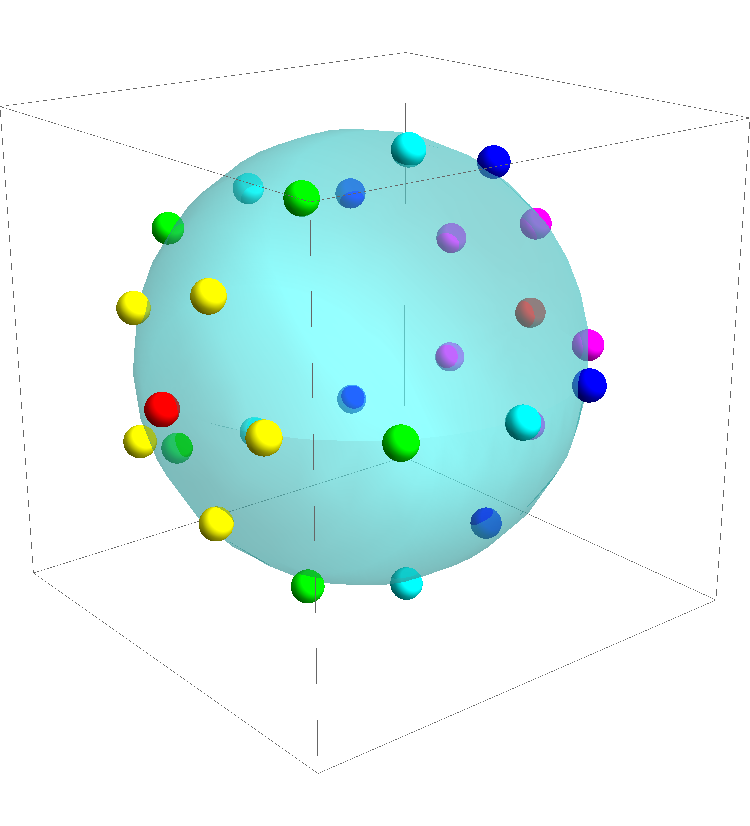
\includegraphics[width=0.48\columnwidth]{hopfS2}}\hfill{}\subfloat[]{\begin{centering}
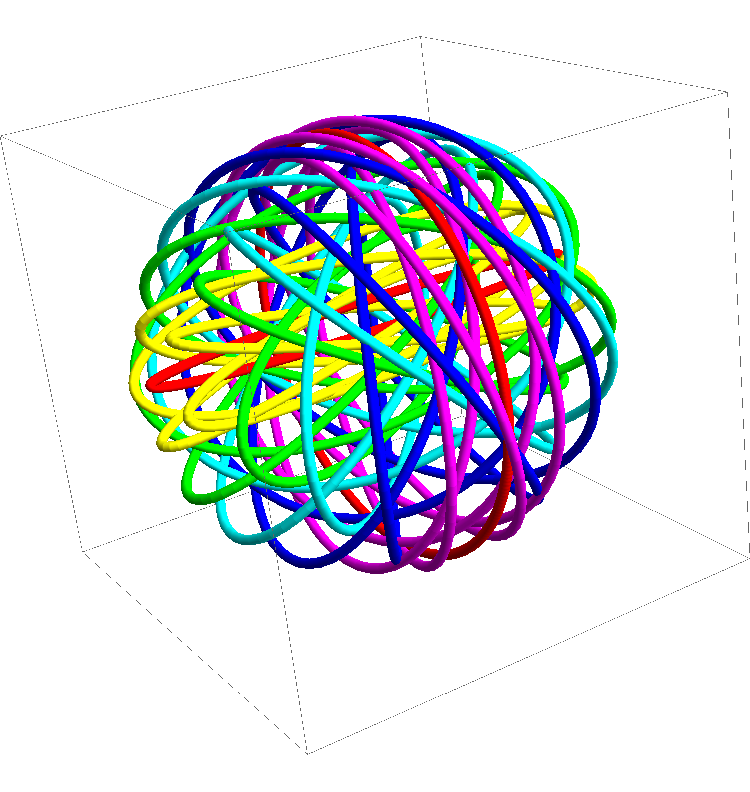
\includegraphics[width=0.48\columnwidth]{hopfFibers}
\par\end{centering}
}\hfill{} \caption{(a) The two-sphere~$\Sphere{2}$ represented by \Eq{A7.eq}, which
is the irreducible space of one-qubit states, along with a representative
set of points on the sphere. Each single point on the sphere in (a)
corresponding to a circle in (b), and a whole family of circles (the
paths of $\rme^{\rmi\theta}$) on the three-sphere~$\Sphere{3}$
represents the Hopf fibration, Eq.~(\ref{eq:HopfFibration}). Although
$\Sphere{3}$ cannot be directly embedded in $\R^{3}$, three-sphere~$\Sphere{3}$
can be regarded as attaching two three-dimensional ball on two sides
of two-sphere~$\Sphere{2}$. In this way, each circle in $\Sphere{3}$
can be represented as a circle in the three-dimensional ball as shown
in (b). Moreover, points in (a) are color coded corresponding to circles
in (b), e.g., one pole contains the red elliptical circle that would
become an infinite-radius circle by a slightly different way to represent
$\Sphere{3}$ in $\R^{3}$, and the opposite pole corresponds to the
large perfectly round red circle at the equator.}
\label{hopfFibers.fig} 
\end{figure}

The resulting manifold is the two-sphere $\Sphere{2}$ (a 2-manifold)
embedded in $\R^{3}$. If we choose one of many possible coordinate
systems describing $\Sphere{3}$ via \Eq{A5.eq} such as 
\begin{equation}
\left(x_{0},y_{0},x_{1},y_{1}\right)=\left(\cos\left(\theta+\phi\right)\cos\psi,\,\sin\left(\theta+\phi\right)\cos\psi,\,\cos\left(\theta-\phi\right)\sin\psi,\,\sin\left(\theta-\phi\right)\sin\psi\right)\,,\label{A8a.eq}
\end{equation}
where %% $0\leq \theta \leq 2 \pi$,  $-\pi \leq \phi \leq  \pi$, 
$0\leq\psi\leq\frac{\pi}{2}$, with $0\leq\theta+\phi<2\pi$ and $0\leq\theta-\phi<2\pi$,
we see that 
\begin{equation}
\left(X,Y,Z\right)=\left(\cos\left(2\phi\right)\sin\left(2\psi\right),\,\sin\left(2\phi\right)\sin\left(2\psi\right),\,\cos\left(2\psi\right)\right)\,.\label{A8b.eq}
\end{equation}
Thus the one-qubit state is independent of $\theta$, and we can choose
$\theta=\phi$ without loss of generality, reducing the form of the
unique one-qubit states to $\ket{\psi_{1}}=\rme^{2\rmi\phi}\cos\psi\ket{0}+\sin\psi\ket{1}$,
and an irreducible state can be represented as a point on a sphere
called the Bloch sphere, as shown in Fig.~\ref{blochSphere.fig}(a).

\begin{figure}[tb]
\begin{centering}
\hfill{}\subfloat[]{\centering{}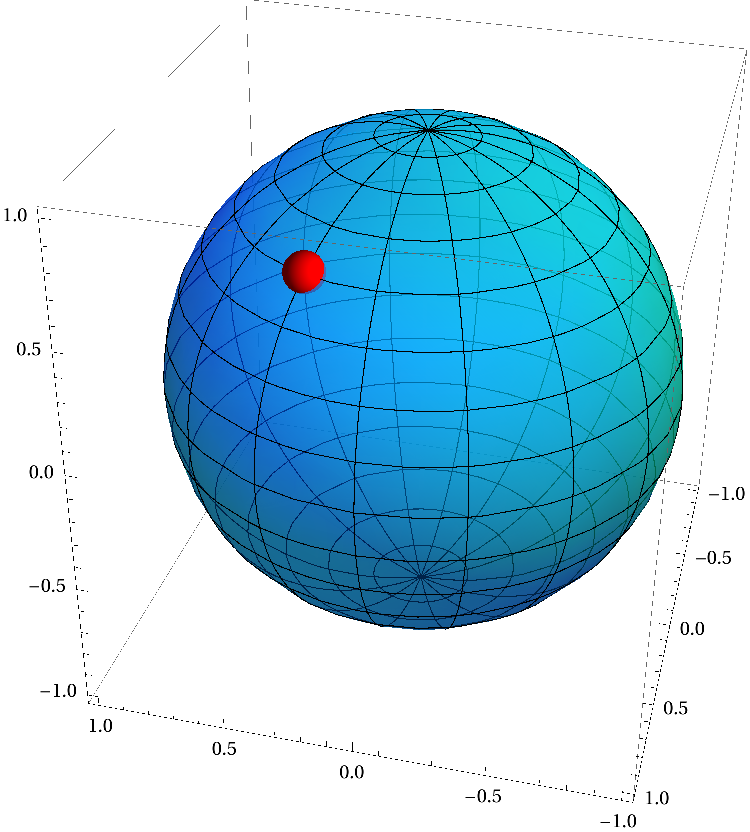
\includegraphics[width=0.47\columnwidth]{blochSphere}}\hfill{}\subfloat[]{\begin{centering}
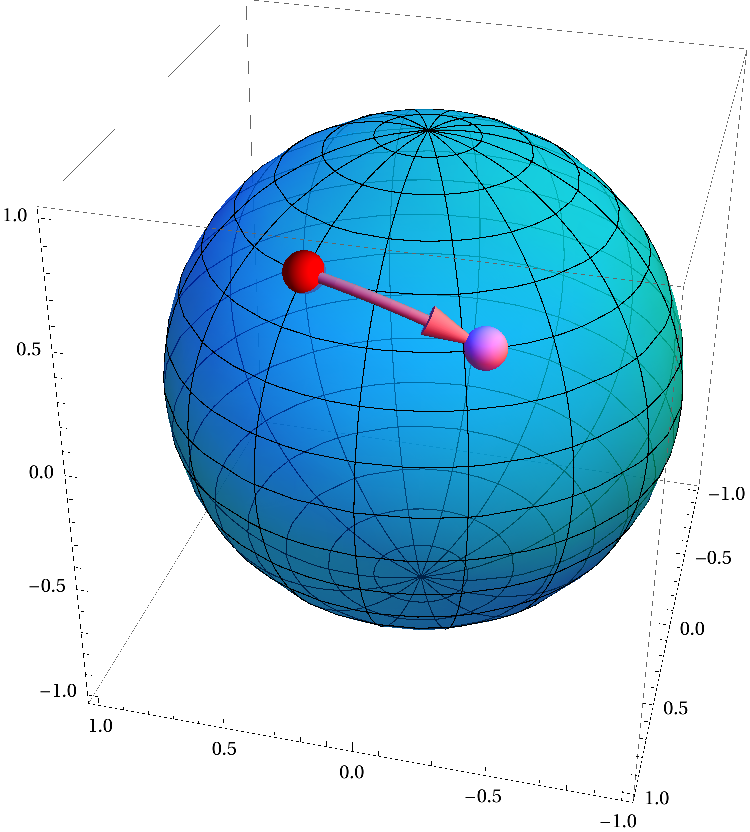
\includegraphics[width=0.47\columnwidth]{blochSphereArc}
\par\end{centering}
}\hfill{}
\par\end{centering}
\caption{(a) The conventional Bloch sphere with a unique state represented
by the point at the red sphere. (b) The geodesic shortest-distance
arc connecting two one-qubit quantum states.}
\label{blochSphere.fig} 
\end{figure}

Thus the geometry of a single qubit reduces to transformations among
points on $\Sphere{2}$, which can be parametrized in an infinite
one-parameter family of transformations, one of which is the geodesic
or minimal-length transformation. Explicitly, given two one-qubit
states denoted by points $\Hat{a}$ and $\Hat{b}$ on $\Sphere{2}$,
the shortest rotation carrying $\Hat{a}$ to $\Hat{b}$ is the SLERP
(spherical linear interpolation) \cite{Shoemake:1985:ARQ:325334.325242,wiki:Slerp}
\begin{equation}
S\left(\Hat{a},\Hat{b},t\right)=\Hat{a}\,\frac{\sin((1-t)\omega)}{\sin\omega}\,+\,\Hat{b}\,\frac{\sin(t\omega)}{\sin\omega}\,,\label{slerp.eq}
\end{equation}
where $\Hat{a}\cdot\Hat{b}=\cos\omega$. Figure \ref{blochSphere.fig}(b)
illustrates the path traced by a SLERP between two irreducible one-qubit
states on the Bloch sphere. Because states in CQC are defined by infinite
precision real numbers, it is not possible, even in principle, to
make an exact state transition as implied by Fig.~\ref{blochSphere.fig}(b).
In practice, one has to be content with approximate, typically exponentially
expensive, transitions from state to state.

\subsection{$D$-dimensional Hilbert Space}

The irreducible states in a $D$-dimensional Hilbert space are encoded
in a similar family of geometric structures known technically as the
complex projective space $\CP{D-1}$. We obtain these structures starting
with the $D$ initially unnormalized complex coefficients of the $D$-dimensional
basis $\ket{\Psi}=\sum_{i=0}^{D-1}\alpha_{i}\ket{i}$. We then follow
the analog of the two-dimensional procedure: Conservation of probability
requires that the norm of the vector $\VVec{\alpha}$ be normalized
to unity: 
\begin{equation}
\braket{\Psi}{\Psi}=\|\VVec{\alpha}\|^{2}=\sum_{i=0}^{D-1}|\alpha_{i}|^{2}=1\,.\label{probEq1.eq}
\end{equation}
Thus the initial equation for the geometry of a quantum state describes
a \textit{topological sphere~}$\Sphere{2D-1}$ embedded in $\mathReal^{2D}$.
To see this, remember that we can write the real and imaginary parts
of $\alpha_{i}$ as $\alpha_{i}=x_{i}+\rmi y_{i}$, so 
\begin{equation}
\sum_{i=0}^{D-1}|\alpha_{i}|^{2}=\sum_{i=0}^{D-1}{x_{i}}^{2}+{y_{i}}^{2}=1
\end{equation}
describes the locus of a $2D$-dimensional real unit vector in $\mathReal^{2D}$,
which is by definition $\Sphere{2D-1}$, the $(2D-1)$-sphere.

This $\Sphere{2D-1}$ in turn is ambiguous up to the usual overall
phase, inducing an $\Sphere{1}$ symmetry action, and identifying
$\Sphere{2D-1}$ as an $\Sphere{1}$ bundle, whose base space is the
$(D-1)$-complex-dimensional projective space $\CP{D-1}$. There are
thus $2D-2$ irreducible real degrees of freedom ($D-1$ complex degrees
of freedom) for a quantum state with a $D$-dimensional basis, $\set{\ket{i}}{i=0,\ldots,D-1}$.

In summary, the full space of a $D$-dimensional quantum state, including
its overall phase defining its relationship to other quantum states,
is the topological space $\Sphere{2D-1}$. For an isolated system,
the overall phase is not measurable, and eliminating the phase dependence
in turn corresponds to identifying $\Sphere{2D-1}$ as a circle bundle
over the base space $\CP{D-1}$, and therefore $\CP{D-1}$ defines
the $2D-2$ intrinsic, irreducible, degrees of freedom of the isolated
$D$-dimensional state's dynamics. In mathematical notation, this
would be written $\Sphere{1}\hookrightarrow\Sphere{2D-1}\rightarrow\CP{D-1}$\todo{Citation?}.
For $D=2$, the single qubit, we have $2-1=1$, and the base space
of the circle bundle is $\CP{1}=\Sphere{2}$, the usual Bloch sphere.
Note that only for $D=2$ is this actually a sphere-like geometry
due to an accident of low-dimensional topology.

\subsection{Explicit generalization of the Hopf fibration construction}

For a two-dimensional system, we could easily solve the problem of
reducing the full unit-norm space to its irreducible components $\Hat{a}=\left(X,Y,Z\right)$
characterizing the Bloch sphere. We have just argued that essentially
the same process is possible for $D$-dimensional system: in the abstract
argument, we simply identify the family of coefficients $\left\{ \alpha_{i}\right\} $
as being the same if they differ only by an overall phase $\rme^{\rmi\theta}$.
However, in practice this is not a construction that is easy to realize
in a practical computation. We now outline an explicit algorithm for
accomplishing the reduction to the irreducible $D$-dimensional state
space $\CP{D-1}$; this construction will turn out to be useful for
the validation of our discrete results to follow below.

Given a normalized pure state $\ket{\Psi}=\sum_{i=0}^{D-1}\alpha_{i}\ket{i}$,
a natural quantity characterizing an $D$-dimensional system is its
\textit{density matrix}, $\rho=\op{\Psi}{\Psi}$, or 
\begin{equation}
\rho=\begin{pmatrix}|\alpha_{0}|^{2} & \alpha_{0}\alpha_{1}^{*} & \cdots & \alpha_{0}\alpha_{D-1}^{*}\\
\alpha_{1}\alpha_{0}^{*} & |\alpha_{1}|^{2} & \cdots & \alpha_{1}\alpha_{D-1}^{*}\\
\vdots & \vdots & \ddots & \vdots\\
\alpha_{D-1}\alpha_{0}^{*} & \cdots & \alpha_{D-1}\alpha_{D-2}^{*} & |\alpha_{D-1}|^{2}
\end{pmatrix}\,.\label{nqDensity.eq}
\end{equation}
We can now use the complex generalization of the classical Veronese
coordinate system for projective geometry to remove the overall phase
ambiguity $\rme^{\rmi\theta}$ from the $D$-dimensional states. If
we take a particular weighting of the elements of the density matrix~$\rho$,
we can construct a \textit{unit vector} of real dimension $D^{2}$
with the form: 
\begin{equation}
\Hat{a}=\left(|\alpha_{i}|^{2},\ldots,\sqrt{2}\,\mathrm{Re}\ \alpha_{i}\alpha_{j}^{*},\ldots,\sqrt{2}\,\mathrm{Im}\ \alpha_{i}\alpha_{j}^{*},\ldots\right)\,,\label{nqCoords.eq}
\end{equation}
where 
\begin{equation}
\Hat{a}\cdot\Hat{a}=\sum_{i=0}^{D-1}\left(\left|\alpha_{i}\right|^{2}\right)^{2}+\sum_{i=0}^{D-1}\sum_{\substack{j=0\\
j\ne i
}
}^{D-1}\left(\mathrm{Re}\ \alpha_{i}\alpha_{j}^{*}\right)^{2}+\left(\mathrm{Im}\ \alpha_{i}\alpha_{j}^{*}\right)^{2}=\left(\sum_{i=0}^{D-1}\left|\alpha_{i}\right|^{2}\right)\left(\sum_{j=0}^{D-1}\left|\alpha_{j}\right|^{2}\right)=1\,.
\end{equation}
This construction gives an explicit embedding of the $\left(D-1\right)$-dimensional
complex, or $\left(2D-2\right)$-dimensional real, object in a real
space of dimension $D^{2}$. However, this is somewhat subtle because
the vector is of unit length, so technically the embedding space is
a sphere of dimension $D^{2}-1$ embedded in $\R^{D^{2}}$. For example,
the two-dimensional irreducible states could be represented in a four-dimensional
embedding, but the magnitude of every coordinate would be one; furthermore,
the object embedded in the resulting $\Sphere{3}$ is indeed $\Sphere{2}$
because we can fix one complex coordinate to be unity, and let one
vary, giving a total of two irreducible dimensions. In fact one must
choose \textit{two} coordinate patches, one covering one pole of $\Sphere{2}$
with coordinates $\alpha_{0}=1+\rmi0$ and $\alpha_{1}=x_{1}+\rmi y_{1}$,
and the other patch covering the other pole of $\Sphere{2}$ with
coordinates $\alpha_{0}=x_{0}+\rmi y_{0}$ and $\alpha_{1}=1+\rmi0$.
\todo{Explain the last part more clear or add a picture.}

We finally see that the irreducible $D$-dimensional state space $\CP{D-1}$
is described by $D$ projectively equivalent coordinates, one of which
can always be scaled out to leave $(D-1)$ actual (complex) degrees
of freedom. We must choose, in turn, $D$ different local sets of
complex variables defined by taking the value $\alpha_{k}=1$, with
$k=0,\ldots,D-1$, and allowing the remaining $D-1$ complex (or $2D-2$
real) variables to run free. No single set of coordinates will work,
since the submanifold including $\alpha_{k}=0$ is undefined and another
coordinate system must be chosen to cover that coordinate patch. This
is a standard feature of the topology of non-trivial manifolds such
as $\CP{D-1}$ (see any textbook on geometry~\cite{Berger_1988}).

\section{Quantum Circuit Model\label{sec:Quantum-Circuit-Model}}

\begin{comment}
An $n$-qubit pure state in the conventional quantum theory (CQT)
is represented as a vector in the $2^{n}$-dimensional Hilbert space.
If we eliminate all symmetries, an irreducible state is actually a
point in the projective Hilbert space \cite{MosseriDandoloff2001,Jaeger2007}
also known as the complex projective space~$\CP{2^{n}-1}$ \cite{Hatcher2001,Bengtsson2007}.
These irreducible quantum states can also be classified as product
states and entangled states, and the latter one plays the essential
role for pure-state algorithms \cite{Mermin2007,Jaeger2007}.
\end{comment}
It has been 36 years since Feynman~\cite{Feynman1982Simulating}
proposed the idea about quantum computation. Although there are many
models for quantum computing, the circuit model is still one of the
most widespread models~\cite{544199} no matter whether in theoretical
study or in building a real quantum computer. Information in a quantum
circuit is stored in qubits. Each qubit is a two-dimensional quantum
system. For a two-qubit system, if the first and second qubit are
described as the state~$\ket{\psi}=\alpha_{0}\ket{0}+\alpha_{1}\ket{1}$
and $\ket{\phi}=\beta_{0}\ket{0}+\beta_{1}\ket{1}$, the state of
the whole system is their tensor product 
\begin{equation}
\begin{aligned} & \ket{\psi}\ket{\phi}=\ket{\psi}\otimes\ket{\phi}=\left(\alpha_{0}\ket{0}+\alpha_{1}\ket{1}\right)\otimes\left(\beta_{0}\ket{0}+\beta_{1}\ket{1}\right)\\
={} & \alpha_{0}\beta_{0}\ket{0}\otimes\ket{0}+\alpha_{0}\beta_{1}\ket{0}\otimes\ket{1}+\alpha_{1}\beta_{0}\ket{1}\otimes\ket{0}+\alpha_{1}\beta_{1}\ket{1}\otimes\ket{1}\\
={} & \alpha_{0}\beta_{0}\ket{0}\ket{0}+\alpha_{0}\beta_{1}\ket{0}\ket{1}+\alpha_{1}\beta_{0}\ket{1}\ket{0}+\alpha_{1}\beta_{1}\ket{1}\ket{1}
\end{aligned}
\end{equation}
in the four-dimensional Hilbert space. For a $n$-qubit system, if
we describe the $j$-th qubit as the state~$\ket{\psi_{j}}$, the
state of the whole system is tensor product of all subsystems $\ket{\Psi}=\ket{\psi_{1}}\otimes\cdots\otimes\ket{\psi_{j}}\otimes\cdots\otimes\ket{\psi_{n}}$
in the Hilbert space of dimension $D=2^{n}$. However, not all quantum
system can be expressed as the tensor product of its subsystems. This
kind of system is called entangled, and will be described in the next
section.\todo{This paragraph need to be polished.}

\subsection{The geometry of entanglement}

\todo{Need to define (partial) trace and mixed state before this
subsection...}

Entanglement may be regarded as one of the main characteristics distinguishing
quantum from classical mechanics. Entanglement involves quantum correlations
such that the measurement outcomes in one subsystem are related to
the measurement outcomes in another one. Within the standard framework,
given a quantum system composed of $n$ qubit subsystems, a pure state
of the total system $\ket{\Psi}$ is said to be entangled if it cannot
be written as a product of states of each subsystem. That is, a state
$\ket{\Psi}$ is entangled if $\ket{\Psi}\ne\ket{\psi_{1}}\otimes\cdots\otimes\ket{\psi_{j}}\otimes\cdots\otimes\ket{\psi_{n}}$,
where $\ket{\psi_{j}}$ refers to an arbitrary state of the $j$-th
qubit, and $\otimes$ represents the tensor product. This is equivalent
to saying that if one calculates the reduced density operator $\rho_{j}$
of the $j$-th subsystem by tracing out all the other subsystems,
$\rho_{j}=\Tr_{\{1,\cdots,j-1,j+1,\cdots,n\}}\left(\rho\right)$,
with $j=1,\cdots,n$ and $\rho=\op{\Psi}{\Psi}$, the normalized state~$\ket{\Psi}$
is entangled if and only if at least one subsystem state is \textit{mixed};
i.e., $\Tr_{j}\left(\rho_{j}^{2}\right)<1$. For example, consider
\begin{equation}
\rho_{j}=\frac{1}{2}\left(\sigma_{0}+\sum\limits _{\mu=x,y,z}\expval{\sigma_{\mu}^{j}}\sigma_{\mu}^{j}\right)\,,
\end{equation}
where $\sigma_{\mu}^{j}$, $\mu=x,y,z$, are the Pauli operators acting
on the $j$-th spin~\cite{544199}, 
\begin{equation}
\sigma_{\mu}^{j}=\overbrace{\sigma_{0}\otimes\cdots\otimes\sigma_{0}\otimes\underbrace{\sigma_{\mu}}_{j^{th}\ \mbox{factor}}\otimes\sigma_{0}\otimes\cdots\otimes\sigma_{0}}^{n\ \mbox{factors}}\,,\label{pauli3}
\end{equation}
with 
\begin{equation}
\begin{aligned}\sigma_{0} & =\left(\begin{array}{cc}
1 & 0\\
0 & 1
\end{array}\right)\,, & \sigma_{x} & =\left(\begin{array}{cc}
0 & 1\\
1 & 0
\end{array}\right)\,, & \sigma_{y} & =\left(\begin{array}{cc}
0 & -\rmi\\
\rmi & 0
\end{array}\right)\,, & \sigma_{z} & =\left(\begin{array}{cc}
1 & 0\\
0 & -1
\end{array}\right)\,,\end{aligned}
\end{equation}
and $\expval{\sigma_{\mu}^{j}}=\melem{\Psi}{\sigma_{\mu}^{j}}{\Psi}$
denotes the corresponding expectation value. The vectors 
\begin{equation}
{\bf X}_{j}=\left(\expval{\sigma_{x}^{j}},\expval{\sigma_{y}^{j}},\expval{\sigma_{y}^{j}}\right)\in\mathbb{R}^{3}
\end{equation}
allow a geometric representation of each reduced state in $\mathbb{R}^{3}$,
satisfying $0\le\left\Vert {\bf X}_{j}\right\Vert \le1$. Since $\Tr_{j}\left(\rho_{j}^{2}\right)=\frac{1}{2}\left(1+\left\Vert {\bf X}_{j}\right\Vert ^{2}\right)$,
the state $\ket{\Psi}$ is entangled if $\left\Vert {\bf X}_{j}\right\Vert <1$
for at least one $j$, represented by a point \emph{inside} the corresponding
local Bloch sphere. One may therefore consider $\ket{\Psi}$ to be
maximally entangled if $\left\Vert {\bf X}_{j}\right\Vert =0$ for
all $j$. On the other hand, the state $\ket{\Psi}$ is unentangled
(i.e., a product state) if $\left\Vert {\bf X}_{j}\right\Vert =1$
for all $j$, corresponding to points lying on the surface of the
Bloch sphere.

A natural geometric measure of multipartite entanglement is obtained
by defining the \emph{purity of a state relative to a set of observables}
\cite{BKOV2003,BKOSV2004}. If the set is chosen to be the set of
\emph{all local observables}, i.e., corresponding to each of the subsystems
that compose the actual system, one recovers the standard notion of
entanglement for multipartite systems. For example, if the system
consists of $n$ qubits, we obtain a measure of conventional entanglement
by calculating the purity relative to the set $\fh=\left\{ \sigma_{x}^{1},\sigma_{y}^{1},\sigma_{z}^{1},\ldots,\sigma_{x}^{n},\sigma_{y}^{n},\sigma_{z}^{n}\right\} $,
\begin{equation}
\begin{aligned}P_{\fh} & =\frac{1}{n}\sum\limits _{j=1}^{n}\sum\limits _{\mu=x,y,z}\expval{\sigma_{\mu}^{j}}^{2}\,, & 0\leq P_{\fh}\leq1\,.\end{aligned}
\label{purityMeasure.eq}
\end{equation}
Since $\fh$ is a semi-simple Lie algebra, its generalized unentangled
states are the generalized coherent states obtained by applying any
group operation to a reference state such as $\ket{\overline{0}}=\ket{0}\otimes\cdots\otimes\ket{0}$.
For the algebra $\fh$ of local observables, such group operations
are simply local rotations on each qubit. In other words, the group
orbit describing the generalized coherent states of $\fh$ comprises
all the product states of the form $\ket{\Psi}=\ket{\psi_{1}}\otimes\cdots\otimes\ket{\psi_{n}}$,
which have maximum purity (i.e., $P_{\fh}=1$). Other states such
as the Greenberger-Horne-Zeilinger state $\ket{\Psi}=\ket{\mathsf{GHZ}_{n}}=\frac{1}{\sqrt{2}}\left(\ket{0}\otimes\cdots\otimes\ket{0}+\ket{1}\otimes\cdots\otimes\ket{1}\right)$
are (maximally) entangled relative to the set of local observables
(i.e., $P_{\fh}=0$).

Different entanglement measures are obtained when a set $\fh$ different
from the local observables is chosen. An obvious example, in particular,
is given by the set of all observables. In this case, the purity takes
its maximum value independently of the pure quantum state \cite{BKOV2003,BKOSV2004},
expressing the fact that any state is a generalized coherent state
of the Lie algebra of all observables.

\subsection{Deutsch Algorithm}

\todo{Further explain $\sigma_{\mu}^{j}$ used as a quantum circuit,
control not, the Deutsch quantum black box~\cite{NCbook}, and maybe
Deutsch Algorithm...}

\section{Quantum Probability\label{sec:fuzzy}}

Given a pure state~$\ket{\phi}$, when we measure an observable represented
by an Hermitian matrix~$\mathbf{O}$, the measurement result is one
of the eigenvalues of $\mathbf{O}$. The probability of getting a
particular eigenvalue~$\lambda$ is $\melem{\phi}{P}{\phi}$, where
$P$ is the projection operator onto the eigenspace of $\lambda$.
This rule of computing the probability is called the Born rule \cite{Born1983,Mermin2007,Jaeger2007},
which is used when we want to extract information from a quantum computer.
For any mixed state~$\rho$, the generalized Born rule induces a
conventional quantum probability measure $\muB_{\rho}:\events\rightarrow[0,1]$,
where $\events$ is the set of all projection operators on a given
Hilbert space. Conversely, any quantum probability measure $\mu:\events\rightarrow[0,1]$
can be induced from a mixed state $\rho$ in the Hilbert space of
dimension $d\ge3$ according to Gleason's theorem \cite{gleason1957,Redhead1987-REDINA,peres1995quantum,RichmanBridges1999,Hamhalter2013}.
In another word, this state $\rho$ is the unique state consistent
with any given quantum probability measure.

\section{Quantum Contextuality}

\todo{Explain enough background knowledge to support the discussion
about contextuality in the end of Sec.~\ref{modalquantum}. I have
typed some literature review in writing course, but I need to decide
whether it could be used or not before finish Sec.~\ref{sec:fuzzy}.}

\chapter{Quantum Theories and Computing over Finite Fields}

\section{Fundamentals of Finite Fields\label{sec:background}}

A field~$\mathbb{F}$ is an algebraic structure consisting of a set
of elements equipped with the operations of addition, subtraction,
multiplication, and division \cite{fieldtheory.ref,numtheory.ref}.
Fields may contain an infinite or a finite number of elements. The
rational~$\mathbb{Q}$, real~$\mathbb{R}$, and complex numbers~$\mathbb{C}$
are examples of infinite fields, while the set $\mathbb{F}_{3}=\{0,1,2\}$,
under multiplication and addition modulo $3$, is an example of a
finite field.

There are two distinguished elements in a field, the addition identity
$0$, and the multiplication identity $1$. Given the field~$\mathbb{F}$,
the closed operations of addition, ``$+$,'' and multiplication,
``$\gmult$,'' satisfy the following set of axioms: 
\begin{enumerate}
\item $\mathbb{F}$ is an Abelian group under the addition operation~$+$
(additive group); 
\item The multiplication operation~$\gmult$ is associative and commutative.
The field has a multiplicative identity and the property that every
nonzero element has a multiplicative inverse; 
\item Distributive laws: For all $a,b,c\in\mathbb{F}$ 
\begin{eqnarray}
a\gmult(b+c) & = & a\gmult b+a\gmult c\\
(b+c)\gmult a & = & b\gmult a+c\gmult a\ .
\end{eqnarray}
\end{enumerate}
\noindent From now on, unless specified, we will omit the symbol~$\gmult$
whenever we multiply two elements of a field.

Finite fields of $q$ elements, $\Fq=\{0,\ldots,q-1\}$, will play
a special role in this work. A simple explicit example is $\mathbb{F}_{3}$
with the following addition and multiplication tables: 
\[
\begin{array}{c|ccc}
+ & 0 & 1 & 2\\[0.1in]
\hline 0 & 0 & 1 & 2\\
1 & 1 & 2 & 0\\
2 & 2 & 0 & 1
\end{array}\hspace*{2cm}\begin{array}{c|ccc}
\gmult & 0 & 1 & 2\\[0.1in]
\hline 0 & 0 & 0 & 0\\
1 & 0 & 1 & 2\\
2 & 0 & 2 & 1
\end{array}
\]

The characteristic of a field is the least positive integer~$m$
such that $m=1+1+1+\cdots+1=0$, and if no such $m$ exists we say
that the field has characteristic zero (which is the case for $\mathbb{R}$
for example). It turns out that if the characteristic is non-zero,
it must be a prime~$p$. For every prime~$p$ and positive integer~$r$
there is a finite field~$\Fpx{p^{r}}$ of size $q=p^{r}$ and characteristic~$p$,
which is unique up to field isomorphism \cite{Artin1991,DummitFoote2004}.
The exponent $r$ is known as the \emph{degree} of the field over
its prime subfield\footnote{ Fields $\ff{q}$ where $q$ is a power of a prime $p$, i.e., $q=p^{r}$,
are known as Galois fields.}~\cite{GT.ref}. If the characteristic $p$ is an arbitrary prime
number, we call the field \emph{unrestricted}.

For every $a\in\Fq$, $a\neq0$, then $a^{q-1}=1$, implying the Frobenius
endomorphism (also a consequence of Fermat's little theorem) $a^{q}=a$,
which in turn permits us to write the multiplicative inverse of any
non-zero element in the field as $a^{-1}=a^{q-2}$, since $a^{q-2}a=a^{q-1}=1$.
Every subfield of the field~$\Fq$, of size $q=p^{r}$, has $p^{r'}$
elements with some $r'$ dividing $r$, and for a given $r'$ it is
unique.

\section{Modal Quantum Theory\label{modalquantum}}

Recently, Schumacher and Westmoreland~\cite{Schumacher2012-SCHMQT,SchumacherWestmoreland2010}
and Chang et al.~\cite{doi:10.1142/S0217984913500644,1751-8121-47-40-405304}
defined versions of quantum theory over \textit{unrestricted} finite
fields, which they call modal quantum theories (MQT) or Galois field
quantum theories. Such theories retain several key quantum characteristics
including notions of superposition, interference, entanglement, and
mixed states, along with time evolution using invertible linear operators,
complementarity of incompatible observables, exclusion of local hidden
variable theories, impossibility of cloning quantum states, and the
presence of natural counterparts of quantum information protocols
such as superdense coding and teleportation. These modal theories
are obtained by collapsing the Hilbert space structure over the field
of complex numbers to that of a vector space over an \emph{unrestricted}
finite field. In the resulting structure, all non-zero vectors represent
valid quantum states, and the evolution of a closed quantum system
is described by \emph{arbitrary} invertible linear maps.

Specifically, consider a one-qubit system with basis vectors $\ket{0}$
and~$\ket{1}$. In conventional quantum theory, there exists an infinite
number of states for a qubit of the form $\alpha_{0}\ket{0}+\alpha_{1}\ket{1}$,
with $\alpha_{0}$ and $\alpha_{1}$ elements of the underlying field
of complex numbers subject to the normalization condition $|\alpha_{0}|^{2}+|\alpha_{1}|^{2}=1$.
Moving to a finite field immediately limits the set of possible states
as the coefficients~$\alpha_{0}$ and~$\alpha_{1}$ are now drawn
from a finite set. In particular, in the field $\ff{2}=\{0,1\}$ of
booleans, there are exactly four possible vectors: the zero vector,
the vector~$\ket{0}$, the vector $\ket{1}$, and the vector $\ket{0}+\ket{1}=\ket{+}$.
Since the zero vector is considered non-physical, a one-qubit system
can be in one of only three states. The dynamics of these one-qubit
states is realized by any invertible linear map, i.e., by any linear
map that is guaranteed never to produce the zero vector from a valid
state. There are exactly $6$ such maps: 
\begin{equation}
\begin{aligned}\sigma_{0} & =\begin{pmatrix}1 & 0\\
0 & 1
\end{pmatrix}\,, & S & =\begin{pmatrix}1 & 0\\
1 & 1
\end{pmatrix}\,, &  & \begin{pmatrix}0 & 1\\
1 & 1
\end{pmatrix}\,,\\
\sigma_{x} & =\begin{pmatrix}0 & 1\\
1 & 0
\end{pmatrix}\,, & S^{\dagger} & =\begin{pmatrix}1 & 1\\
0 & 1
\end{pmatrix}\,, &  & \begin{pmatrix}1 & 1\\
1 & 0
\end{pmatrix}\,.
\end{aligned}
\end{equation}
This set of maps is clearly quite impoverished compared to the full
set of one-qubit unitary maps in conventional quantum theory. In particular,
it does not include the Hadamard transformation. However, this set
also includes non-unitary maps such as $S$ and $S^{\dagger}$ that
are not allowed in conventional quantum computation.

Measurement in the standard basis is fairly straightforward: measuring
$\ket{0}$ or $\ket{1}$ deterministically produces the same state
while measuring $\ket{+}$ nondeterministically produces $\ket{0}$
or $\ket{1}$ with no assigned probability distribution. When measuring
an arbitrary state~$\ket{\phi}\in\left\{ \ket{0},\ket{1},\ket{+}\right\} $
in other bases $\left\{ \ket{\psi_{0}},\ket{\psi_{1}}\right\} $,
we first represents $\ket{\phi}$ as the linear combination of the
basis vectors $\beta_{0}\ket{\psi_{0}}+\beta_{1}\ket{\psi_{1}}$,
where $\beta_{0}$ and $\beta_{1}$ are elements in the field~$\ff{2}$.
If $\beta_{i}$ is zero, measuring $\ket{\phi}$ is impossible to
produce $\ket{\psi_{i}}$; otherwise, measuring $\ket{\phi}$ is possible
to produce $\ket{\psi_{i}}$. Since only possibility and impossibility
is predicted by the theory, modal quantum theories are named after
these “modal” concepts.

Notice that the measurement process is complicated by the fact that
the possibility to produce a basis vector~$\ket{\psi_{i}}$ depending
on the measurement basis. For example, measuring $\ket{+}$ is possible
to produce $\ket{0}$ in the standard basis $\left\{ \ket{0},\ket{1}\right\} $
but is impossible to produce $\ket{0}$ in another basis $\left\{ \ket{+},\ket{0}\right\} $.
In contrast, when measuring a state~$\ket{\phi}$ in CQT, the probability
to produce a basis vector~$\ket{\psi_{i}}$ is completely determined
by $\ket{\psi_{i}}$ and $\ket{\phi}$ no matter $\ket{\psi_{i}}$
is in which measurement basis. This phenomena of the measurement basis
dependence in CQT only exists when discussing quantum contextuality.
Despite this kind of ``supercontextuality'' of MQT, its computational
model, modal quantum computing (MQC), having ``supernatural'' computational
power is also far from conventional quantum computing as we will describe
next.

\section{Modal Quantum Computing\label{modalquantumcomputing}}

To understand the computational implications of the modal quantum
theory defined over the field $\ff{2}$ of booleans, we developed
a quantum computing model and established its correspondence to a
classical model of logical programming with a feature that has quantum-like
behavior~\cite{finiteQC}. In a conventional logic program, answers
produced by different execution paths are collected in a sequence
with \emph{no} interference. However, in this modal quantum computing
model over $\ff{2}$, these answers may interfere destructively with
one another.

Our computations with this ``toy'' modal quantum theory showed that
it possesses ``supernatural'' computational power. For example,
one can solve a black box version of the \usat\ problem~\cite{usat}
in a way that outperforms conventional quantum computing. The classical
\usat\ problem (also known as $\lang{USAT}$ or $\lang{UNAMBIGUOUS-SAT}$\todo{Add
citation about where these two names come from.}) is the problem
of deciding whether a given boolean formula has a satisfying assignment,
assuming that it has at most one such assignment~\cite{Papadimitriou1993}.
This problem is, in a precise sense~\cite{Valiant198685}, just as
hard as the general satisfiability problem and hence all problems
in the~NP complexity class. Our black-box version of the \usat\ problem
replaces the boolean formula with an arbitrary black box. Solutions
to this generalized problem can be used to solve an unstructured database
search of size $N$ using $O\left(\log N\right)$ black box evaluations
by binary search on the database. This algorithm then outperforms
the known asymptotic bound $O\left(\sqrt{N}\right)$ for unstructured
database search in conventional quantum computing.

\begin{figure}[t]
\[
\xyR{.9em}\xyC{.6em}\entrymodifiers={@*=<0em>}\xymatrix{\lstick{y=\ket{0}} & \qw & \multigate{3}{\uf} & \gate{~S^{\dagger}~} & \ctrl{3} & \gate{~S^{\dagger}~} & \multimeasureD{3}{\text{measure}}\\
\lstick{x_{1}=\ket{0}} & \multigate{2}{\otimes S} & \ghost{\uf} & \multigate{2}{\otimes S} & \targ & \qw & \ghost{\text{measure}}\\
\lstick{\ldots} & \ghost{\otimes S} & \ghost{\uf} & \ghost{\otimes S} & \targ & \qw & \ghost{\text{measure}}\\
\lstick{x_{n}=\ket{0}} & \ghost{\otimes S} & \ghost{\uf} & \ghost{\otimes S} & \targ & \qw & \ghost{\text{measure}}
}
\]
\caption{\label{fig:alg}Circuit for black box \usat\ in modal quantum theory
over the field $\ff{2}$. $\uf$ is a Deutsch quantum black box~\cite{544199}
with $\uf\ket{y}\ket{\overline{x}}~=~\ket{y\scalarPlus f(\overline{x})}\ket{\overline{x}}$,
where $\overline{x}$ denotes a sequence $x_{1},x_{2},\ldots,x_{n}$
of $n$ bits. For further notation see text.}
\end{figure}

We can prove the unreasonable power of the arbitrary-function \usat\ starting
with a classical function $f:\boolt^{n}\rightarrow\boolt$ that takes
$n$ bits and returns at most one \btrue\ result. Then we can give
an algorithm (see Fig.~\ref{fig:alg}) taking as input such a classical
function that decides, deterministically and in a constant number
of black box evaluations, whether $f$ is satisfiable or not:

\paragraph*{Case I: $f$ is unsatisfiable; the measurement deterministically
produces $\ket{0}\ket{\overline{0}}$.}

The state is initialized to $\ket{0}\ket{\overline{0}}$, with $\ket{\overline{0}}=\ket{0}\ket{0}\cdots\ket{0}$,
i.e., the tensor product of $n$ $\ket{0}$ states. Applying the map
$S$ (defined in the previous section) to each qubit in the second
component of the state produces $\ket{0}\ket{\overline{+}}$ where
$\ket{\overline{+}}$ denotes the sequence $\ket{+}\ldots\ket{+}$
of length $n$. Applying $\uf$ to the entire state has no effect
since $U_{f}$ is the identity when $f$ is unsatisfiable. Applying
$S$ to each qubit in the second component of the state produces $\ket{0}\ket{\overline{0}}$.
Applying $S^{\dagger}$ to the first component leaves the state unchanged.
As the first component of the state is 0, applying the map $X_{0}$
(which is the identity) leaves the state unchanged. Applying $S^{\dagger}$
to the first component leaves the state unchanged. Measuring the state
will deterministically produce $\ket{0}\ket{\overline{0}}$.

\paragraph*{Case II: $f$ is satisfiable; the measurement produces some state
other than $\ket{0}\ket{\overline{0}}$.}

Assume the function $f$ is satisfiable at some input $a_{1},a_{2},\ldots,a_{n}$
denoted $\overline{a}$, and where $\ket{\overline{a}}=\ket{a_{1}}\ldots\ket{a_{n}}$.
In the second step, the state becomes $\ket{0}\ket{\overline{+}}$
as above. We can write this state as $\ket{0}\ket{\overline{a}}+\Sigma_{\overline{x}\neq\overline{a}}\ket{0}\ket{\overline{x}}$.
Applying $U_{f}$ produces $\ket{1}\ket{\overline{a}}+\Sigma_{\overline{x}\neq\overline{a}}\ket{0}\ket{\overline{x}}$.
We can rewrite this state as $\ket{+}\ket{\overline{a}}+\Sigma_{\overline{x}}\ket{0}\ket{\overline{x}}=\ket{+}\ket{\overline{a}}+\ket{0}\ket{\overline{+}}$,
where the summation is now over all vectors (notice that $\ket{0}\ket{\overline{a}}+\ket{0}\ket{\overline{a}}$
is the zero vector). Applying $S$ to each qubit in the second component
produces $\ket{+}\ket{\overline{S(a)}}+\ket{0}\ket{\overline{0}}$.
Applying $S^{\dagger}$ to the first component produces: $\ket{1}\ket{\overline{S(a)}}+\ket{0}\ket{\overline{0}}$.
Applying $X_{b}$, where $b$ is the first component of the state,
to each qubit in the second component produces $\ket{1}\ket{\overline{{\sf not}(S(a))}}+\ket{0}\ket{\overline{0}}$.
Applying $S^{\dagger}$ to the first component produces $\ket{+}\ket{\overline{{\sf not}(S(a))}}+\ket{0}\ket{\overline{0}}$.
For the measurement of $\ket{+}\ket{\overline{{\sf not}(S(a))}}+\ket{0}\ket{\overline{0}}$
to be guaranteed to never be $\ket{0}\ket{\overline{0}}$, we need
to verify that $\ket{+}\ket{\overline{{\sf not}(S(a))}}$ has one
occurrence $\ket{0}\ket{\overline{0}}$. This can be easily proved
as follows. Since each $a_{i}$ is either 0 or 1, then each $S(a_{i})$
is either $+$ or $1$, and hence each ${\sf not}(S(a_{i}))$ is either~$+$
or~$0$. The result follows since any state with a combination of
$+$ and $0$, when expressed in the standard basis, would consist
of a superposition containing the state $\ket{0\ldots}$.

\begin{comment}

\section{Modal Quantum Theory and Computing}

Our first discrete model replaces the complex numbers by a unrestricted
finite field~$\mathbb{F}_{q}$ \cite{Schumacher2012-SCHMQT,DQT2014,SchumacherWestmoreland2010}.
In this model, an $n$-qubit state is a non-zero vector in $\mathbb{F}_{q}^{2^{n}}$.
When we measure a given state~$\ket{\phi}$, an observable is replaced
by a basis~$\mathcal{B}$ of $\mathbb{F}_{q}^{2^{n}}$. Since $\ket{\phi}$
can be represented by the summation across a unique subset~$\mathcal{S}$
of the basis~$\mathcal{B}$, whether it is possible or impossible
to measure a basis vector~$\ket{i}$ depends on whether $\ket{i}$
is in $\mathcal{S}$ or not. Because this model only predicts whether
a result is possible or impossible, it is called the modal quantum
theory. Its computational model, called the modal quantum computing,
is far from conventional quantum computing. Although modal quantum
computing can express simple algorithms such as quantum teleportation
\cite{BennettBrassardEtAl1993,peres1995quantum,Mermin2007,Jaeger2007},
it is so weak that it cannot express Deutsch's algorithm \cite{Deutsch1985,Mermin2007}.
This quantum theory is, however, also so powerful that it can be used
to solve an unstructured database search of size $N$ using $O(\log(N))$
steps, which outperforms the known asymptotic bound $O(\sqrt{N})$
in conventional quantum computing \cite{Grover:1996:FQM:237814.237866,BennettBernsteinBrassardVazirani1997,Mermin2007,Jaeger2007}.
\end{comment}

\section{Discrete Quantum Theory (I)\label{discretequantumtheoryI}}

Our next objective is to develop more realistic discrete quantum theory
variants that exclude ``supernatural'' algorithms such as the one
presented above. Our first such plausible framework~\cite{powerdqc}
is based on complexifiable finite fields. To incorporate complex numbers
for quantum amplitudes, we exploit the fact that the polynomial $x^{2}+1=0$
is \emph{irreducible} (has no solution) over a prime field $\ff{p}$
with $p$ odd if and only if $p$ is of the form~$4\ell+3$, with
$\ell$ a non-negative integer. In other words, $x^{2}+1=0$ is irreducible
over $\ff{3},\ff{7},\ff{11},\ff{19},\ldots$. We achieve our goal
by observing that any field in this family is extensible to a field~$\ff{p^{2}}$
whose elements can be viewed as discrete complex numbers with the
real and imaginary parts in~$\ff{p}$. In the field~$\ff{p^{2}}$,
the Frobenius automorphism of an element $\alpha$ (defined as $\alpha^{p}$)
represents the usual definition of complex conjugation~\cite{fieldexample}.

The next task is to examine the consequences when we attempt to construct
$d$-dimensional vector spaces over the complexified fields $\ff{p^{2}}$
\cite{geom1}. (For readability, instead of writing column vectors,
we will often use the vector notation $\ket{\Psi}=(\alpha_{0}~\alpha_{1}~\ldots~\alpha_{d-1})^{T}$
and $\ket{\Phi}=(\beta_{0}~\beta_{1}~\ldots~\beta_{d-1})^{T}$, where
$(.)^{T}$ is the transpose of the \textit{row} vector $(.)$.) It
can be shown~\cite{HermitianProd} that, given two vectors 
\begin{equation}
\ket{\Psi}=\sum_{i=0}^{d-1}~\alpha_{i}\ket{i}\ ,\ \ket{\Phi}=\sum_{i=0}^{d-1}~\beta_{i}\ket{i},
\end{equation}
with scalars $\alpha_{i}$ and $\beta_{i}$ drawn from the field elements,
and orthonormal basis $\{\ket{i}\}$, the Hermitian \dotprod\ is
always reducible to the form \vspace{-0.1in}
 
\begin{equation}
\ip{\Phi}{\Psi}=\sum_{i=0}^{d-1}~\beta_{i}^{p}~\alpha_{i}^{\;}\ .\vspace{-0.1in}\label{innerprod}
\end{equation}

This product satisfies conditions A and B below, but not~C, because
in a finite field, addition can ``wrap around,'' making the concepts
of positive and negative meaningless and allowing the sum of non-zero
elements to be zero: 
\begin{itemize}
\item A. $\ip{\Phi}{\Psi}$ is the complex conjugate of $\ip{\Psi}{\Phi}$;
\vspace*{-0.25cm}
 
\item B. $\ip{\Phi}{\Psi}$ is conjugate linear in its first argument and
linear in its second argument; \vspace*{-0.25cm}
 
\item C. $\ip{\Psi}{\Psi}$ is always non-negative and is equal to~0 only
if $\ket{\Psi}$ is the zero vector. 
\end{itemize}
With just conditions A and B, it is possible to recover unitary operators,
and thus recover much of the relevant structure of Hilbert spaces
over the field of complex numbers. The failure of condition C, however,
plays havoc with the traditional notions of ordered probabilities
as well as the geometric notions of ordered distances and angles,
whose lengths and cosines, respectively, are normally expressed using
the inner product~\cite{geom}. In a separate development, we explore
the geometry of these finite fields and define a discrete version
of the Hopf fibration extending the Bloch sphere to $n$-qubits, as
well as determining discrete measures for the relative sizes of the
entangled, maximally entangled, and unentangled discrete states~\cite{geom1}.

\begin{comment}

\section{Vector Spaces over Complexified Finite Fields}

In order to address the intrinsic problems induced by the notion of
the continuum calculations of the previous section, one is led to
replace the infinite fields of CQC by discrete computable fields.
Accomplishing this while maintaining the essential elements of addition
and multiplication requires a brief excursion into the theory of fields,
and particularly the theory of finite fields.

\subsection{Background}

Abstract algebra deals with various kinds of algebraic structures,
such as groups, rings, and fields, each defined by a different system
of axioms. A field~$\mathbf{F}$ is an algebraic structure consisting
of a set of elements equipped with the operations of addition, subtraction,
multiplication, and division \cite{numtheory.ref}. Fields may contain
an infinite or a finite number of elements. The rational $\mathbb{Q}$,
real $\mathbb{R}$, and complex numbers $\mathbb{C}$ are examples
of infinite fields, while the set $\mathbf{F}_{3}=\{0,1,2\}$ under
the usual multiplication and modular addition is an example of a finite
field. Finite fields are also known as Galois fields \cite{GT.ref}.

There are two distinguished elements in a field, the addition identity
$0$, and the multiplication identity $1$. Given the field $\mathbf{F}$,
the closed operations of addition, ``$+$'', and multiplication,
``$\gmult$'', satisfy the following set of axioms:
\begin{enumerate}
\item $\mathbf{F}$ is an Abelian group under the addition operation $+$
(additive group)
\item The multiplication operation $\gmult$ is associative and commutative.
The field has a multiplicative identity and the property that every
nonzero element has a multiplicative inverse
\item Distributive laws: For all $a,b,c\in\mathbf{F}$ 
\begin{eqnarray}
a\gmult(b+c)=a\gmult b+a\gmult c\\
(b+c)\gmult a=b\gmult a+c\gmult a\ .
\end{eqnarray}
\end{enumerate}
{}From now on, unless specified, we will omit the symbol $\gmult$
whenever we multiply two elements of a field.

Finite fields of $q$ elements, $\Fq=\{0,\ldots,q-1\}$, will play
a special role in this work. A simple explicit example is the following
addition and multiplication tables for $\mathbf{F}_{3}$: 
\[
\begin{array}{c|ccc}
+ & 0 & 1 & 2\\[0.1in]
\hline 0 & 0 & 1 & 2\\
1 & 1 & 2 & 0\\
2 & 2 & 0 & 1
\end{array}\hspace*{2cm}\begin{array}{c|ccc}
\gmult & 0 & 1 & 2\\[0.1in]
\hline 0 & 0 & 0 & 0\\
1 & 0 & 1 & 2\\
2 & 0 & 2 & 1
\end{array}
\]

\subsection{Cyclic Properties of Finite Fields}

Finite fields are classified by size. The characteristic of a field
is the least positive integer $m$ such that $m=1+1+1+\cdots+1\equiv0$,
and if no such $m$ exists we say that the field has characteristic
zero (which is the case for infinite fields such as $\mathbb{R}$).
It turns out that if the characteristic is non-zero it must be a prime
$p$. For every prime $p$ and positive integer $r$ there is a finite
field $\Fpx{p^{r}}$ of cardinality $q=p^{r}$ and characteristic
$p$ (Lagrange's theorem), which is unique up to field isomorphisms.
For every $a\in\Fq$, $a\neq0$, then $a^{q-1}=1$, implying the Frobenius
endomorphism (also a consequence of Fermat's little theorem) $a^{q}=a$,
which in turn permits us to write the multiplicative inverse of any
non-zero element in the field as $a^{-1}=a^{q-2}$, since $a^{q-2}a=a^{q-1}=1$.
Every subfield of the field $\Fq$, of cardinality $q=p^{r}$, has
$p^{r'}$ elements with some $r'$ dividing $r$, and for a given
$r'$ it is unique. Notice that a fundamental difference between finite
and infinite fields is one of topology: finite fields induce a compact
structure because of their modular arithmetic, permitting \textit{wrapping
around}, while that is not the case for fields of characteristic zero.
This feature may lead to fundamental physical consequences.

\subsection{Complexified Finite Fields}

Consider the polynomial $x^{2}+1=0$ over a finite field $\Fp$. It
is known that this polynomial does not have solutions in the field
precisely when the prime $p$ is congruent to $3\imod{4}$ (see, e.g.,
\cite{numtheory.ref}).

For such primes, it is therefore possible to construct an extended
field $\Fpp$ whose elements are of the form $\alpha=a+ib$ with $a\in\Fp$,
$b\in\Fp$, and $i$ the root of the polynomial $x^{2}+1=0$. Since
the field elements $a+ib$ behave like discrete versions of the complex
numbers, we will refer to fields $\Fp$ with prime $p$ congruent
to $3\imod{4}$ as \emph{complexifiable finite fields}, and $i$-extended
fields $\Fpp$ with $p$ congruent to $3\imod{4}$ as \emph{complexified
finite fields}.

In a complexified finite field $\Fpp$, the Frobenius automorphism
that maps $\alpha\in\Fpp$ to $\alpha^{p}\in\Fpp$ acts like complex
conjugation. For example, in $\Fppx{3}$, we have $(2+i)^{3}=8+12i-6-i=2+11i$
which, in the field, is equal to $2-i$ since $11\equiv-1\imod{3}$.

We define the \emph{field norm} $\fnorm{\cdot}$ as the map from $(a+ib)\in\Fpp$
to $a^{2}+b^{2}\in\Fp$, 
\begin{equation}
\fnorm{\alpha=a+ib}=a^{2}+b^{2}\ .\label{fieldnorm.eq}
\end{equation}
We avoid the square root in the discrete field framework because,
unlike the continuous case, the square root does not always exist.

\subsection{Vector Spaces}

In this section we want to build a theory of discrete vector spaces
that approximates as closely as possible the features of conventional
quantum theory. Such a structure would ideally consist of the following:
(i) a vector space over the field of complex numbers, and (ii) an
inner product $\ip{\Phi}{\Psi}$ associating to each pair of vectors
a complex number, and satisfying the following properties: 
\begin{itemize}
\item[A.] $\ip{\Phi}{\Psi}$ is the complex conjugate of $\ip{\Psi}{\Phi}$; 
\item[B.] $\ip{\Phi}{\Psi}$ is conjugate linear in its first argument and
linear in its second argument; 
\item[C.] $\ip{\Psi}{\Psi}$ is always non-negative and is equal to~0 only
if $\ket{\Psi}$ is the zero vector. 
\end{itemize}
It turns out that a vector space defined over a finite field cannot
have an inner product satisfying the properties above. However, we
will introduce an Hermitian ``dot product'' satisfying some of those
properties.

We are interested in the $n$-qubit vector space ${\cal H}$ of dimension
$D=2^{n}$ defined over the complexified field $\Fpp$. Let $\ket{\Psi}=(\alpha_{0}~\alpha_{1}~\ldots~\alpha_{D-1})^{T}$
and $\ket{\Phi}=(\beta_{0}~\beta_{1}~\ldots~\beta_{D-1})^{T}$ represent
vectors in ${\cal H}$, with numbers $\alpha_{i}$ and $\beta_{i}$
drawn from $\Fpp$, and where $(\cdot)^{T}$ is the transpose.

\begin{definition}{[}Hermitian dot product{]} Given vectors $\ket{\Phi}$
and $\ket{\Psi}\in{\cal H}$, the Hermitian dot product of these vectors
is: 
\begin{equation}
\ip{\Phi}{\Psi}=\sum_{i=0}^{D-1}~\beta_{i}^{p}~\alpha_{i}^{\;}\ .
\end{equation}
\end{definition} Two vectors $\ket{\Phi}$ and $\ket{\Psi}\in{\cal H}$
are said to be orthogonal if $\ip{\Phi}{\Psi}=0$. This product satisfies
conditions A and B for inner products but violates condition C since
in every finite field there always exists a non-zero vector $\ket{\Psi}$
such that $\ip{\Psi}{\Psi}=0$. The reason is that addition in finite
fields eventually ``wraps around'' (because of their cyclic or modular
structure), allowing the sum of non-zero elements to be zero. The
fraction of non-zero vectors satisfying $\ip{\Psi}{\Psi}=0$ decreases
with the order $p$.

For any vector $\ket{\Psi}=(\alpha_{0}~\alpha_{1}~\ldots~\alpha_{D-1})^{T}$,
the Hermitian dot product $\ip{\Psi}{\Psi}$ is equal to $\sum_{i=0}^{D-1}~\fnorm{\alpha_{i}}$,
which is the sum of the field norms for the complex coefficients.
For convenience, we now extend the field norm to include vector arguments
by defining 
\begin{equation}
\fnorm{\ket{\Psi}}=\ip{\Psi}{\Psi}=\sum_{i=0}^{D-1}~\fnorm{\alpha_{i}}\ .\label{fnormD.eq}
\end{equation}
The field norm of a vector can vanish for non-vanishing vectors.

For vectors $\ket{\Psi}$ such that $\ip{\Psi}{\Psi}=\sum_{i=0}^{D-1}\alpha_{i}^{p}\,\alpha_{i}^{\;}=\sum_{i=0}^{D-1}\alpha_{i}^{p+1}=\sum_{i=0}^{D-1}|\alpha_{i}|^{2}$
has a square root in the field, one can define the following ``norm'':
\begin{equation}
||\Psi||=\sqrt{\ip{\Psi}{\Psi}}\ ,\label{norm-eq}
\end{equation}
which is valid only on a subspace of the field norm for finite fields.

%There is an alternative way of defining a proper inner product over a subset of the %field $\Fpp$. Consider prime numbers $p= 8 \prod_{l=1}^k q_l -1$, where  %$q_l$ are odd primes. This subset of the primes congruent to $3 \imod 4$ has the %special properti

\section{Irreducible Discrete $n$-qubit States: Generalized Discrete Bloch
Sphere}

\label{DQCnqubitBloch.sec}

In the one-qubit state with coefficients in $\Fpp$, the discrete
analog of the Bloch sphere is constructed by exact analogy to the
continuous case: we first require that the coefficients of the single
qubit basis obey 
\begin{equation}
\|\psi_{1}\|^{2}=|\alpha_{0}|^{2}+|\alpha_{1}|^{2}=1\label{DQA2.eq}
\end{equation}
in the discrete field. In \ref{appU.sec}, we show that there are
$p(p^{2}-1)$ such values. Given this requirement, which is similar
in form to the conservation of probability, but not as useful due
to the lack of orderable probability values, we can immediately conclude
that the discrete analog of the Hopf fibration is again 
\begin{eqnarray}
X & = & 2\,\mathrm{Re}\ \alpha_{0}\alpha_{1}^{*}=2x_{0}x_{1}+2y_{0}y_{1}\nonumber \\
Y & = & 2\,\mathrm{Im}\ \alpha_{0}\alpha_{1}^{*}=2x_{1}y_{0}-2x_{0}y_{1}\label{DQA6.eq}\\
Z & = & |\alpha_{0}|^{2}-|\alpha_{1}|^{2}=x_{0}^{\ 2}+y_{0}^{\ 2}-x_{1}^{\ 2}-y_{1}^{\ 2}\ ,\nonumber 
\end{eqnarray}
but now with all computations in $(\mbox{mod}~p)$. At this point
one simply writes down all possible discrete values for the complex
numbers $\{\alpha_{0},\alpha_{1}\}$ satisfying Eq.~(\ref{DQA2.eq})
and enumerates those that project to the same value of $\{X,Y,Z\}$.
This equivalence class is the discrete analog of the circle in the
complex plane that was eliminated in the continuous case. In \ref{appH.sec},
we show that $p+1$ discrete values of $\{\alpha_{0},\alpha_{1}\}$
with unit norm map to the same point under the Hopf map \Eq{DQA6.eq};
we may think of these as discrete circles or projective lines of equivalent,
physically indistinguishable, complex phase. The surviving $p(p-1)$
values of $\{\alpha_{0},\alpha_{1}\}$ correspond to irreducible physical
states of the discrete single qubit system. %% Several examples are shown in Figure \ref{bloch.fig}. %%Thus,
for example, choosing the underlying field to be $\Fppx{3}$, there
are exactly 6 single-qubit state vectors to populate the Bloch sphere;
the four equivalent phase-multiples mapping to each of the six points
on the $\Fppx{3}$ Bloch sphere are collapsed and regarded as physically
indistinguishable. In Figure \ref{bloch.fig}, we plot the irreducible
states on the Bloch sphere for $p=3$, $7$, and $11$. Note that
the Cartesian lengths of the real vectors corresponding to the points
on the Bloch sphere vary considerably due to the nature of discrete
fields; we have artificially normalized them to a ``continuous world''
unit radius sphere for conceptual clarity.

\begin{figure}[htb]
%\vspace{-0.2in}  %% \includegraphics[width=0.9\columnwidth]{./Bloch_sphere.pdf}%%\includegraphics[width=2.0\columnwidth]{./picA.png}%%\includegraphics[width=2.0\columnwidth]{./picB.png}

\begin{centering}
\hspace*{-0.5cm}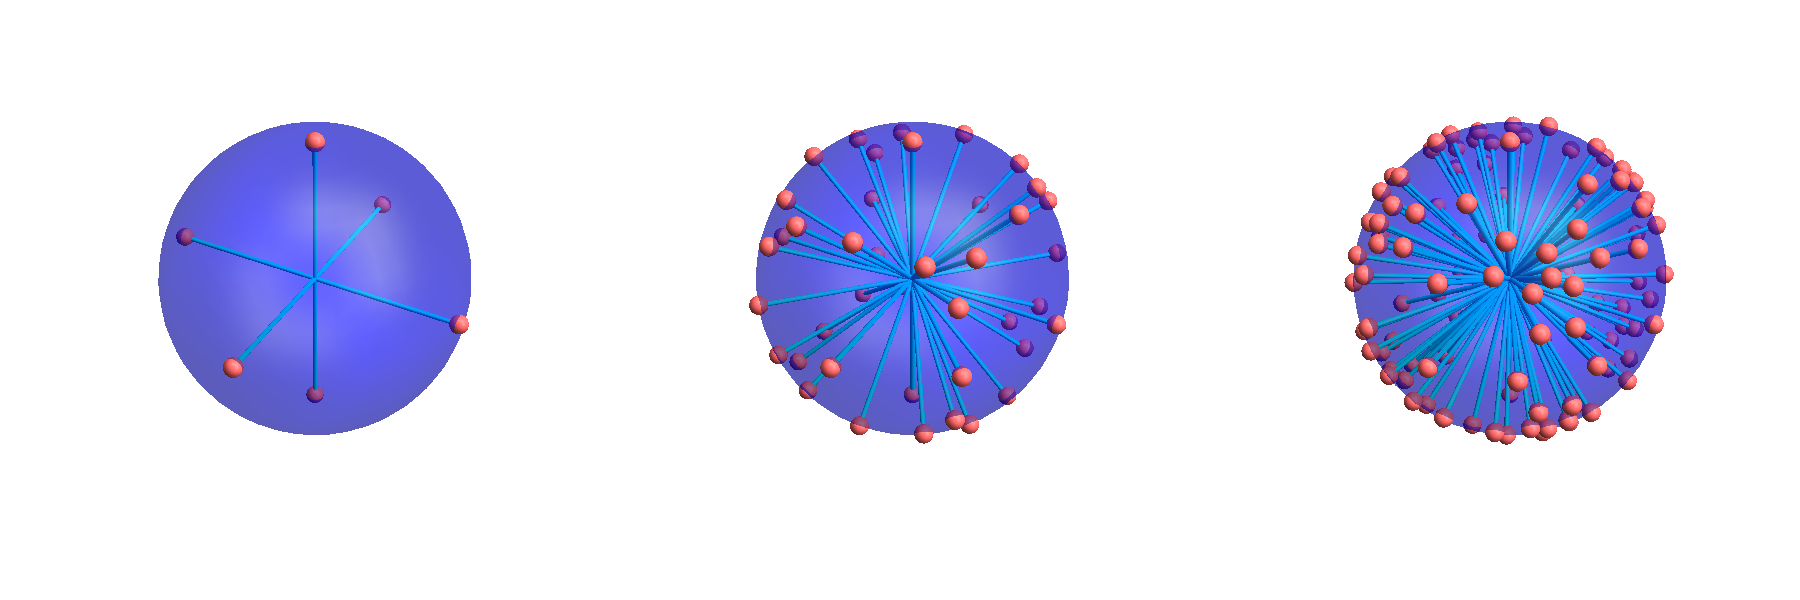
\includegraphics[width=1.1\columnwidth]{../../../Public/Documents/StudyInIUB/Computer Science/201209-12.M800/Manuscripts/picC.png}
%%\includegraphics[width=0.5\textwidth]{./picAB.eps}\vspace{-0.2in}
 %% adjust blank space?
\par\end{centering}
\caption{Schematically normalized plots of the elements of the discrete Bloch
sphere, the irreducible single-qubit (two-dimensional) state vectors
with unit norm over the field $\Fpp$. We show the results for $p=3$,
$7$, and $11$. For example, in $\Fppx{3}$, there are 24 vectors
of unit norm, but only the 6 inequivalent classes appear in the plot.
The $p+1=4$ equivalent vectors in each class differ only by a complex
discrete phase.}
\label{bloch.fig} 
\end{figure}

\subsection{Counting states on the $n$-qubit Bloch sphere}

We have the unique opportunity in the finite-field approach to quantum
computing to precisely identify and enumerate the physical states.
In the conventional theory, as we have seen, we employ a generalized
Hopf fibration on the normalized states to project out a circle of
phase-equivalent states, yielding the generalized Bloch sphere.

In the introduction to this section, we sketched the counting of the
irreducible single-qubit discrete states. To count the number of inequivalent
discrete states for the general $n$-qubit case with coefficients
in $\Fpp$, we first must find the set of unit-norm states, and then
determine the equivalence classes of unit-norm states under discrete
phase transformations; we can then enumerate the list of states on
the discrete generalized Bloch sphere. By executing computer searches
of these spaces, we discovered an hypothesis for a closed-form solution
for the counting of the states, and were then able to find a rigorous
inductive proof of the enumeration, which is presented in the Appendix.

This process of describing the discrete $n$-qubit irreducible states
can again be understood geometrically by following the discrete analog
of the Hopf fibration. First, we construct the discrete version of
the quadratic unit-length form that automatically annihilates the
distinction among states differing only by a discrete phase, 
\begin{eqnarray}
\hspace*{-0.5cm}\Hat{a}=(|\alpha_{i}|^{2},...,\sqrt{2}\ \mathrm{Re}\ \alpha_{i}\alpha_{j}^{*},\ldots,\sqrt{2}\ \mathrm{Im}\ \alpha_{i}\alpha_{j}^{*},\ldots)\ ,
\end{eqnarray}
where 
\begin{eqnarray}
\Hat{a}\cdot\Hat{a}=\left(\sum_{i=0}^{D-1}\left|\alpha_{i}\right|^{2}\right)^{2}=1\ .
\end{eqnarray}
{}From \ref{appH.sec}, we know that $p+1$ elements of this discrete
$\Sphere{2\times2^{n}-1}$ structure map to the \textit{same point\/}
in $\Hat{a}$. Each set of $(p+1)$ redundant points is, geometrically
speaking, the \textit{discrete Hopf fibration circle\/} living above
each \textit{irreducible\/} point of the $n$-qubit state description.
These $p+1$ points are interpretable as the $p$ finite points plus
the single point at infinity of the projective discrete line (see,
e.g., \cite{Arnold}).

The next part of this argument is the determination of the unit-norm
states, effectively the space of allowed discrete partitions of unity;
we cannot exactly call these ``probability-conserving'' sectors
of the state coefficients since we do not have a well defined notion
of probability, but we do have a well-defined notion of partition
of unity. The tally of unit-norm states is $p^{2^{n}-1}(p^{2^{n}}-1)$
(see \ref{appU.sec}) compared to the total number $p^{2\times2^{n}}$
of possible complex integer state vectors that could be chosen. This
unit-norm state structure is the discrete analog of $\Sphere{2\times2^{n}-1}$.

Finally, we repeat the last step of the $n$-qubit continuous Hopf
fibration process for discrete $n$-qubit states, eliminating the
discrete set of $p+1$ equivalent points that map to the same point
$\Hat{a}$ on the generalized $n$-qubit Bloch sphere. Dividing the
tally $p^{2^{n}-1}(p^{2^{n}}-1)$ of unit norm states by the $p+1$
elements of each phase-equivalent discrete circle, we find 
\[
\frac{p^{2^{n}-1}(p^{2^{n}}-1)}{p+1}=p^{2^{n}-1}(p-1)\,\prod_{k=1}^{n-1}(p^{2^{k}}+1)
\]
as the total count of unique irreducible states in a discrete $n$-qubit
configuration (see \ref{appI.sec}). The resulting object is precisely
the discrete version of $\CP{D-1}$, which we might call a \textit{discrete
complex projective space\/} or $\DCP{D-1}$, where $D=2^{n}$ as
usual.

\Comment{ 

\subsection{Counting states on the $n$-qubit Bloch sphere}

Although we do not have a rigorous proof for the counting of discrete
unit-norm states and the number of irreducible unit-norm states in
the discrete generalized Bloch sphere for $n$-qubit states with coefficients
in $\Fpp$, we have run extensive computer searches of the state features
for a range of compatible primes $p$ and number of qubits $n$. From
these experimental investigations, we have induced a closed-form solution
for the counting that agrees for every possible combination of parameters
that can be computed in reasonable time (the computational complexity
becomes intractable very quickly).

For $n$-qubit discrete states with coefficients in $\Fpp$, our calculation
begins with an enumeration of all possible $2^{n}$-tuples of state
coefficients in $\Fpp$; then the moduli-squared of these tuples are
summed and compared to unity in $(\mbox{mod}~p)$. Those that survive
are accumulated in a list of allowed discrete partitions of unity;
we cannot exactly call these ``probability-conserving'' sectors
of the state coefficients since we do not have a well defined notion
of probability, but we do have a well-defined notion of partition
of unity. The heuristic number that results for the tally of unit-norm
states is $p^{2^{n}-1}(p^{2^{n}}-1)$, compared to the total number
$p^{2\times2^{n}}$ of possible complex integer state vectors that
could be chosen. This unit-norm state structure is now the discrete
analog of $\Sphere{2\times2^{n}-1}$.

Finally, we construct the discrete version of the quadratic unit-length
form that automatically annihilates the distinction among states differing
only by a discrete phase, 
\begin{eqnarray}
\hspace*{-0.5cm}\Hat{a}=\{|\alpha_{i}|^{2},...,\sqrt{2}\ \mathrm{Re}\ \alpha_{i}\alpha_{j}^{*},\ldots,\sqrt{2}\ \mathrm{Im}\ \alpha_{i}\alpha_{j}^{*},\ldots\}\ ,
\end{eqnarray}
where 
\begin{eqnarray}
\Hat{a}\cdot\Hat{a}=\left(\sum_{i=0}^{D-1}\left|\alpha_{i}\right|^{2}\right)^{2}=1\ .
\end{eqnarray}
Computing all the elements of the discrete $\Sphere{2\times2^{n}-1}$
structure that map to the \textit{same point\/} in $\Hat{a}$, we
find a $(p+1)$-fold redundancy, exactly as for the one-qubit case;
each set of $(p+1)$ redundant points is, geometrically speaking,
the \textit{discrete Hopf fibration circle\/} (see, e.g., Arnold
\cite{Arnold}) living above each \textit{irreducible\/} point of
the $n$-qubit state description.

In summary, when the $n$-qubit continuous Hopf fibration process
is repeated for the discrete analog of $n$-qubit states, we find
that that analog of a phase ``circle'' is a discrete set $p+1$
equivalent points that map to the same point $\Hat{a}$ on the generalized
$n$-qubit Bloch sphere, and therefore there are a total of $p^{2^{n}-1}(p^{2^{n}}-1)/(p+1)$
unique irreducible states in a discrete $n$-qubit configuration.
The resulting object is precisely the discrete version of $\CP{D-1}$,
which we might call a \textit{discrete complex projective space\/}
or $\DCP{D-1}$. }

\section{Geometry of Entangled States}

Without regard to uniqueness, an $n$-qubit state with discrete complex
coefficients in $\Fpp$ will have the total possible space of coefficients
with dimension $p^{2\times2^{n}}$ (including the null state). Imposing
the condition of a length-one norm %% AMR: replaced 'inner-product' by 'norm'in
$\Fp$, this number is reduced to $p^{2^{n}-1}(p^{2^{n}}-1)$. The
ratio of all the states to the unit-norm states is asymptotically
$p$: 
\begin{eqnarray}
\frac{p^{2^{n}+1}}{p^{2^{n}}-1}\rightarrow p\ ,
\end{eqnarray}
so there are roughly $p$ sets of coefficients, for any number of
qubits $n$, that are discarded for each retained unit-length state
vector. A factor of $p+1$ more states are discarded in forming the
discrete Bloch sphere of irreducible states. Selected plots of the
full space compared to both the unit-norm space and the irreducible
space for a selection of complexified finite fields are shown in Figure
\ref{statePlot3Unit.fig} for 1, 2, 3, and 4 qubits. %Figure \ref{statePlot3Unit.fig} adds the size of the irreducible state%space at the bottom.

%% Source of this is%%  ~hansona/home2/papers/dqc-geom-2012/00mathFigs/A-Test-Galois-Nqubit.nb

%\begin{figure}[htb]%\begin{center}%\includegraphics[width=1.0\columnwidth]{./statePlot1.pdf}%%\vspace{-0.2in}  %% adjust blank space?%\end{center}% \caption{Logarithmic plot of the number of discrete unnormalized%states (top, in red), vs the number of normalized discrete states%(bottom, in blue) for the first 6 $\Fpp$-compatible primes,  (3, 7,%11, 19, 23, 31), for the number of qubits 1, 2, 3 and 4. }% \label{statePlotUnit.fig}%\end{figure}

\begin{figure}[htb]
\begin{centering}
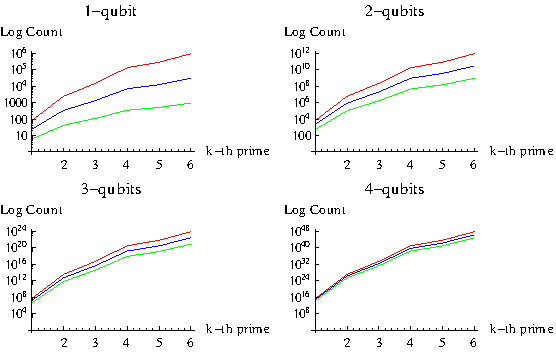
\includegraphics[width=1\columnwidth]{../../../Public/Documents/StudyInIUB/Computer Science/201209-12.M800/Manuscripts/statePlot3.pdf}
%\vspace{-0.2in}  %% adjust blank space?
\par\end{centering}
\caption{Logarithmic plot of the number of discrete unnormalized states (top,
in red), vs the number of normalized discrete states (middle, in blue),
vs the irreducible states (bottom, in green) for the first 6 $\Fpp$-compatible
primes, (3, 7, 11, 19, 23, 31), for the number of qubits 1, 2, 3 and
4. }
\label{statePlot3Unit.fig} 
\end{figure}

\subsection{Unentangled vs Entangled Discrete States}

For a given $p$ and the corresponding complexified field $\Fpp$,
the $n$-qubit discrete quantum states with coefficients in $\Fpp$
can be classified by their degree of entanglement to a level of precision
that is unavailable in the continuous theory. We look first at the
unentangled $n$-qubit states, which are direct product states of
the form 
\begin{equation}
\ket{\Psi}=\ket{\psi_{1}}\otimes\cdots\otimes\ket{\psi_{j}}\otimes\cdots\otimes\ket{\psi_{n}}\ .\label{dqcNqUntg.eq}
\end{equation}
Without regard to normalization, there are $(p^{4})^{n}$ possible
unentangled states out of the total of $p^{2\times2^{n}}$ states
noted above. When we normalize the individual product states to unit
norm, the norm of the entire $n$-qubit state becomes the product
of those unit norms, and is automatically normalized to one. We have
already seen that each single-qubit normalized state in the tensor
product \Eq{dqcNqUntg.eq} has precisely $p(p-1)$ irreducible components.

\subsection{Completely Unentangled States and the Discrete Bloch Sphere}

In effect, the irreducible states for unentangled $n$-qubit configurations
reduce to a single Bloch sphere for each one-qubit component $\ket{\psi_{j}}$,
and thus the whole set of states is defined by an $n$-tuple of discrete
Bloch sphere coordinates. Since each Bloch sphere in $\Fpp$ has $p(p-1)$
distinct irreducible components, we have 
\[
\mbox{{\bf Count of Unentangled States}}=p^{n}(p-1)^{n}\ .
\]

We know that the total number of irreducible states (points in the
generalized $\DCP{2^{n}-1}$ Bloch sphere) for an $n$-qubit state
is $p^{2^{n}-1}(p^{2^{n}}-1)/(p+1)$, and so the number of states
containing some measure of entanglement is 
\begin{eqnarray*}
\mbox{{\bf Count of Entangled States}}=\frac{p^{2^{n}-1}(p^{2^{n}}-1)}{p+1}-p^{n}(p-1)^{n}\ .
\end{eqnarray*}
Therefore a very small fraction of the unit norm states are unentangled.

\subsection{Partial entanglement}

A partially entangled state can be constructed by taking individual
component states to enter as direct products, starting by picking
$n$ distinct single qubits to be unentangled ($n=2$ exhausts its
freedom with one pick). Then we can choose $n(n-1)/2$ pairs of distinct
qubits as product states ($n=3$ exhausts its freedom with one pick),
and so on. Then, starting with $n=3$, we can pick fully entangled
2-qubit subspaces as product spaces, combining them with single-qubit
product components ($n=3$ has no single-qubit freedom left after
picking any of its three 2-qubit subspaces), and so on. Precise measures
of entanglement such as that given in \Eq{purityMeasure.eq} can
then be applied just as in the continuous case.

\subsection{Maximal entanglement}

Numerical and analytic calculations of the entanglement measure \Eq{purityMeasure.eq},
taken $(\mbox{mod}~p)$, extend to the best of our knowledge to the
discrete case, so that the unentangled states constructed above have
$P_{\fh}=1$. This leads us to study one final aspect of the discrete
$n$-qubit states, namely the \textit{maximally\/} entangled states
with $P_{\fh}=0$.

Computing some examples for various $n$ and small values of $p$,
one can verify explicitly that unit-norm unentangled states for $n=2$,
$p=\{3,7,11,19,\ldots\}$ occur with frequency 
\[
(p+1)p^{2}(p-1)^{2}=\{144,14112,145200,2339280,\ldots\}\ ,
\]
and for general $n$, $(p+1)p^{n}(p-1)^{n}$.

The irreducible state counts are reduced by $(p+1)$, giving 
\[
p^{2}(p-1)^{2}=\{36,1764,12100,116964,\ldots\}\ ,
\]
and in general for $n$-qubits, $p^{n}(p-1)^{n}$ instances of pure
states with $P_{\fh}=1$.

Repeating the computation to discover the frequency of maximally entangled
(purity $P_{\fh}=0$ states), we find $p^{n+1}(p-1)(p+1)^{n}$ maximally
entangled states, with example frequencies for two qubits of 
\[
p^{3}(p-1)(p+1)^{2}=\{864,131712,1916640,49384800,\ldots\}\ .
\]

The irreducible state counts for maximal entanglement are reduced
by $(p+1)$, giving for $n=2$ 
\[
p^{3}(p^{2}-1)=\{216,16464,159720,2469240,\ldots\}\ ,
\]
and in general for $n$-qubits, $p^{n+1}(p-1)(p+1)^{n-1}$ instances
of pure states with $P_{\fh}=0$.

Therefore, the ratio of maximally entangled to unentangled states
is 
\[
\mbox{{\bf Max Entangled/Unentangled}}=p\left(\frac{p+1}{p-1}\right)^{n-1}\ .
\]

\section{Summary}

Given a discrete basis for the complex coefficients of an $n$-qubit
quantum state, DQC permits us in principle to explicitly determine
the relative frequencies of phases and to determine exactly the generalized
Bloch sphere coordinates of the irreducible states. The size of the
set of states that must be taken as equivalent to get irreducibility
is the size of the ``circle'' or phase group, and this is $p+1$
for any $p$ and for any $n$ (related to the size of the finite projective
line, see \cite{Arnold}). Exploring the discrete manifestation of
the purity measure \Eq{purityMeasure.eq}, our DQC approach can determine
not only the size of the irreducible space of states, but also the
relative sizes of the unentangled and entangled states for $n$ discrete
qubits.

\vspace{0.5in}

\noindent \textbf{References} \vspace*{0.5cm}

\bibitem{GeomQStates2008} I. Bengtsson and K. Zyczkowski, \textit{Geometry
of Quantum States: An Introduction to Quantum Entanglement} (Cambridge
University Press, Cambridge, 2008). 

\bibitem{mosseri2001} R. Mosseri and R. Dandoloff, \textit{J. Phys.
A: Math. Gen.} \textbf{34}, 10243 (2001). 

\bibitem{Arnold} V. I. Arnold, \textit{Dynamics, Statistics and Projective
Geometry of Galois Fields\/} (Cambridge University Press, Cambridge,
2011). 

\bibitem{Turing37} A. M. Turing, \textit{Proceedings of the London
Mathematical Society} Series 2, \textbf{42}, 230 (1937). Errata appeared
in Series 2, \textbf{43} 544 (1937). 

\bibitem{Minsky67} M. Minsky, \textit{Computation: Finite and Infinite
Machines} (Prentice-Hall, Englewood Cliffs, 1967). See chapter 9,
``The Computable Real Numbers.'' 

\bibitem{Chaitin} G. J. Chaitin, \textit{Thinking about Gödel and
Turing} (World Scientific, Singapore, 2007). 

\bibitem{Feynman} R. P. Feynman, \textit{Int. J. Theor. Phys.} \textbf{21},
467 (1982). 

\bibitem{Landauer} R. Landauer, \textit{Physics Letters A\/} \textbf{217},
188 (1996). 

\bibitem{SchuWest2010} B. Schumacher and M. D. Westmoreland, \textit{Found.
Phys. \/} \textbf{42}, 918 (2012). 

\bibitem{James2011} R. P. James, G. Ortiz, and A. Sabry, \texttt{http://arxiv.org/abs/1101.3764}. 

\bibitem{HOSW2011} A. J. Hanson, G. Ortiz, A. Sabry, and J. Willcock,
\texttt{http://arxiv.org/abs/1104.1630}. 

\bibitem{Berger} M. Berger and B. Gostiaux, \textit{Differential
Geometry: Manifolds, Curves, and Surfaces\/} (Springer-Verlag, New
York, 1988). 

\bibitem{numtheory.ref-1} G. H. Hardy and E. M. Wright, \textit{An
Introduction to the Theory of Numbers\/} (Oxford University Press,
Oxford, 2006). 

\bibitem{GT.ref-1} I. Stewart, \textit{Galois theory\/} (Chapman
and Hall/CRC, Boca Raton, 2004). \Comment{ 

\bibitem{WB.ref} Wildberger N J 2005 \textit{Divine Proportions:
Rational Trigonometry to Universal Geometry} (Sydney: Wild Egg Books) 

\bibitem{OT} Ovsienko V and Tabachnikov S 2005 \textit{Projective
Differential Geometry Old and New} (Cambridge: Cambridge University
Press) 

\bibitem{VY} Veblen O and J. W. Young J W 1946 \textit{Projective
Geometry Vol. 2} (Blaisdell Publishing Company), pp 55??7 

\bibitem{Ztransform} Campello de Souza R M, de Oliveira H M and Silva
D 2002 The Z Transform over Finite Fields \textit{International Telecommunications
Symposium, ITS 2002, Brazil} } 

\bibitem{Barnum2003} H. Barnum, E. Knill, G. Ortiz, and L. Viola,
\textit{Phys. Rev. A} \textbf{68}, 032308 (2003). 

\bibitem{Barnum2004} H. Barnum, E. Knill, G. Ortiz, R. Somma, and
L. Viola, \textit{Phys. Rev. Lett.} \textbf{92}, 107902 (2004). 
\end{comment}

\section{Discrete Quantum Computing (I)\label{discretequantumcomputingI}}

Given a complexified finite field $\ff{p^{2}}$ and its Hermitian
\dotprod\
(Eq.~\eqref{innerprod}) much of the structure of conventional quantum
computing can be recovered. For example, the smallest field~$\ff{3^{2}}$
is already rich enough to express the standard Deutsch-Jozsa~\cite{NCbook}
algorithm, which requires only normalized versions of vectors or matrices
with the scalars $0$, $1$, and $-1$. Similarly, other deterministic
quantum algorithms (algorithms for which we may determine the outcome
with certainty), such as Simon's and Bernstein-Vazirani, perform as
desired~\cite{simon}. Algorithms such as Grover's search will not
work in the usual way because we lack (the notion of) ordered angles
and probability in general.

\begin{figure}[t]
\[
\xyR{.9em}\xyC{.6em}\entrymodifiers={@*=<0em>}\xymatrix{\lstick{y=\ket{0}} & \qw & \multigate{3}{\uf} & \qw & \multimeasureD{3}{\text{measure}}\\
\lstick{x_{1}=\ket{0}} & \multigate{2}{H} & \ghost{\uf} & \multigate{2}{H} & \ghost{\text{measure}}\\
\lstick{\ldots} & \ghost{H} & \ghost{\uf} & \ghost{H} & \ghost{\text{measure}}\\
\lstick{x_{n}=\ket{0}} & \ghost{H} & \ghost{\uf} & \ghost{H} & \ghost{\text{measure}}
}
\]
\caption[]{Circuit for black box \usat\ in discrete quantum computing.}
\label{fig:dbsearch} 
\end{figure}

It is possible, in some situations, to exploit the cyclic behavior
of the field to creatively cancel probability amplitudes and solve
problems with what again appears to be ``supernatural'' efficiency.
We illustrate this behavior with the algorithm in Fig.~\ref{fig:dbsearch},
which is a variant of the one in Fig.~\ref{fig:alg}. Unlike the
modal quantum theory algorithm, the new algorithm does not always
succeed deterministically using a constant number of black box evaluations.
We can, however, show that supernatural behavior occurs if the characteristic
$p$ of the field divides $2^{N}-1$. For a database of fixed size
$N$, matching the conditions becomes less likely as the size of the
field increases. Nevertheless, for a \textit{given\/} field, it is
always possible to expand any database with dummy records to satisfy
the divisibility property. Physically, we are taking advantage of
additional interference processes that happen because of the possibility
of ``wrapping around'' due to modular arithmetic. We do not know,
in general, whether this version of discrete quantum computing actually
enables the rapid solution of NP-complete problems

.%
\begin{comment}

\section{Discrete Quantum Theory and Computing (I)}

Our second model called discrete quantum theory (I) considers only
finite fields of order $p^{2}$, with the prime $p$ of the form $4\ell+3$
($\ell$ a non-negative integer) \cite{geometry2013,DQT2014}. In
this model, an irreducible state is a vector in $\mathbb{F}_{p^{2}}^{2^{n}}$,
and can be reduced to a point in the discrete complex projective space~$\mathbb{DCP}^{2^{n}-1}$.
Among these irreducible states, the product states and entangled states
can not only be identified as in CQT but also be counted for different
$p$. Although the state space is a natural discrete analog to CQT,
this model still only predicts whether a measurement result is possible
or impossible, because it is not possible to define an inner product
in the usual sense due to the modular arithmetic~\cite{grove2002classical}.
Under suitable conditions, we can have deterministic quantum algorithms
such as the algorithms of Deutsch, Simon \cite{Simon:1994:PQC:1398518.1399019,Mermin2007,Jaeger2007},
and Bernstein-Vazirani \cite{Bernstein:1993:QCT:167088.167097,Mermin2007},
but this still leads to excessive computational power for the unstructured
database search problem for certain database sizes.
\end{comment}

\section{Discrete Quantum Theory and Computing (II)}

Our third model, discrete quantum theory (II)~\cite{DQT2014}, restricts
states in some local region of $\mathbb{F}_{p^{2}}^{2^{n}}$. Within
a local region, a notion of inner product and probability could be
recovered. Its discrete quantum computing can be further applied to
the deterministic Deutsch-Jozsa algorithm \cite{DeutschJozsa1992,Jaeger2007}
and the probabilistic Grover algorithm \cite{Grover:1996:FQM:237814.237866,Mermin2007,Jaeger2007}.

\section{Toward Discrete Quantum Probability}

When people tried to define quantum probability over finite fields,
people tended to treat the original Born rule as an axiom, and tried
to modify it to get a discrete Born rule \cite{Schumacher2012-SCHMQT,doi:10.1142/S0217984913500644,DQT2014,Ellerman2016a}.
However, any modified Born rule could hardly work on the whole vector
space, since there is no inner product on the whole vector space over
finite fields. Instead of treating the Born rule as an axiom, the
Born rule can actually be deduced from a set of abstract definitions
and axioms according to Gleason's theorem. Although we might hope
to deduce a discrete Born rule directly from a similar set of definitions
and axioms, no discrete Born rule satisfies certain properties motivated
by Gleason's theorem with infinitely precise real-number probability~\cite{Gardiner2014}.
Since the state spaces are now discrete and finite, this suggests
us to consider a discrete Born rule mapping to finite number of intervals
called interval-valued probability~\cite{JamisonLodwick2004,THOS2017}.
To adopting the idea of interval-valued probability step-by-step,
before attempting to study quantum interval-valued probability over
finite fields, we will first review the classical interval-valued
probability, and extend it with the conventional quantum theory.

\chapter{Quantum Interval-Valued Probability}

\section{Classical Interval-Valued Probability}

In the classical setting, there are several proposals for ``imprecise
probabilities'' \cite{Shafer1976,GilboaSchmeidler1994,Marinacci1999,JamisonLodwick2004,HuberRonchetti2009,Grabisch2016}.
Although these proposals differ in some details, they all share the
fact that the probability $\bar{\mu}(E)$ of an event~$E$ is generalized
from a single \emph{real number} to an \emph{interval}~$[l,r]$,
where~$l$ intuitively corresponds to the strength of evidence for
the event~$E$ and~$1-r$ corresponds to the strength of evidence
against the same event. Given a sample space~$\Omega$ and a set
of intervals~$\mathscr{I}$, similar to a classical probability measure
$\mu:2^{\Omega}\rightarrow\left[0,1\right]$, a classical interval-valued
probability measure (IVPM) $\bar{\mu}:2^{\Omega}\rightarrow\mathscr{I}$
needs to satisfy some coherent axioms. By satisfying the convexity
axiom \cite{Shapley1971,GilboaSchmeidler1994,Marinacci1999,Grabisch2016},
Shapley proved that there is always a classical probability measure
consistent with the classical IVPM~$\bar{\mu}$ \cite{Shapley1971,GilboaSchmeidler1994,Grabisch2016}.
Given any random variable, its expectation value with respect to classical
probability measures consistent with~$\bar{\mu}$ is consistent with
its Choquet integral \cite{Choquet1954,GilboaSchmeidler1994,Grabisch2016}
with respect to $\bar{\mu}$ \cite{Rosenmuller1971,GilboaSchmeidler1994,Grabisch2016}.

\section{Quantum Interval-Valued Probability}

The quantum extension, quantum interval-valued probability measure
(QIVPM) $\bar{\mu}:\events\rightarrow\mathscr{I}$, is a generalization
of both classical IVPMs $\bar{\mu}:2^{\Omega}\rightarrow\mathscr{I}$
and conventional quantum probability measures $\mu:\events\rightarrow[0,1]$
\cite{THOS2017}, because QIVPMs reduce to classical IVPMs when the
space of quantum events $\events$ is restricted to mutually commuting
events, and reduces to conventional quantum probability measures when
mapping to infinitely precise uncountable intervals $\mathscr{I}_{\infty}=\set{\left[x,x\right]}{x\in\left[0,1\right]}$.
While Shapley and Gleason both proved there must be a ``state''
consistent with any given QIVPM in the reduced cases, in general there
exists a QIVPM such that no state is consistent with it. However,
we found a class of QIVPMs such that all QIVPMs in this class are
consistent with a non-empty ``ball'' of quantum states whose radius
is defined by the maximal length of the intervals, and recovers the
original Gleason theorem asymptotically. Similarly, the conventional
quantum expectation value and the classical Choquet integral are together
generalized to the quantum interval-valued expectation value. This
is used to prove an imprecise Kochen-Specker theorem \cite{BELL_1966,kochenspecker1967,Redhead1987-REDINA,peres1995quantum,Jaeger2007}
which suggests a possible resolution of the Meyer-Mermin debate on
the impact of finite-precision measurement on the Kochen-Specker theorem
\cite{PhysRevLett.83.3751,Mermin1999}.

\chapter{Further Questions}

When people proved the original Gleason theorem, people usually exploited
the geometrical structure of real 3-dimensional Hilbert space \cite{gleason1957,peres1995quantum,RichmanBridges1999,Hamhalter2013}.
Since our finite-precision extension of the Gleason theorem only applies
on a class of QIVPMs, we might want to ask how to modify these geometrical
arguments to have a Gleason-type theorem for general QIVPMs. We will
further study the tensor product structure among QIVPMs which is essential
for defining product and entangled states, and serves the basis to
discuss quantum nonlocality~\cite{Bell1964,Redhead1987-REDINA,peres1995quantum,Jaeger2007}
and quantum computing with QIVPMs. Finally, we want to improve the
discrete quantum theories to consider QIVPMs over finite fields in
future research.

\addcontentsline{toc}{chapter}{Bibliography} %
\begin{comment}
 \bibliographystyle{plain}
\bibliography{prop}
\end{comment}
\printbibliography

% http://latex.org/forum/viewtopic.php?t=7312
% http://latex.org/forum/viewtopic.php?t=17956
\addtocontents{toc}{\contentsline{chapter}{Curriculum Vitae}{}}
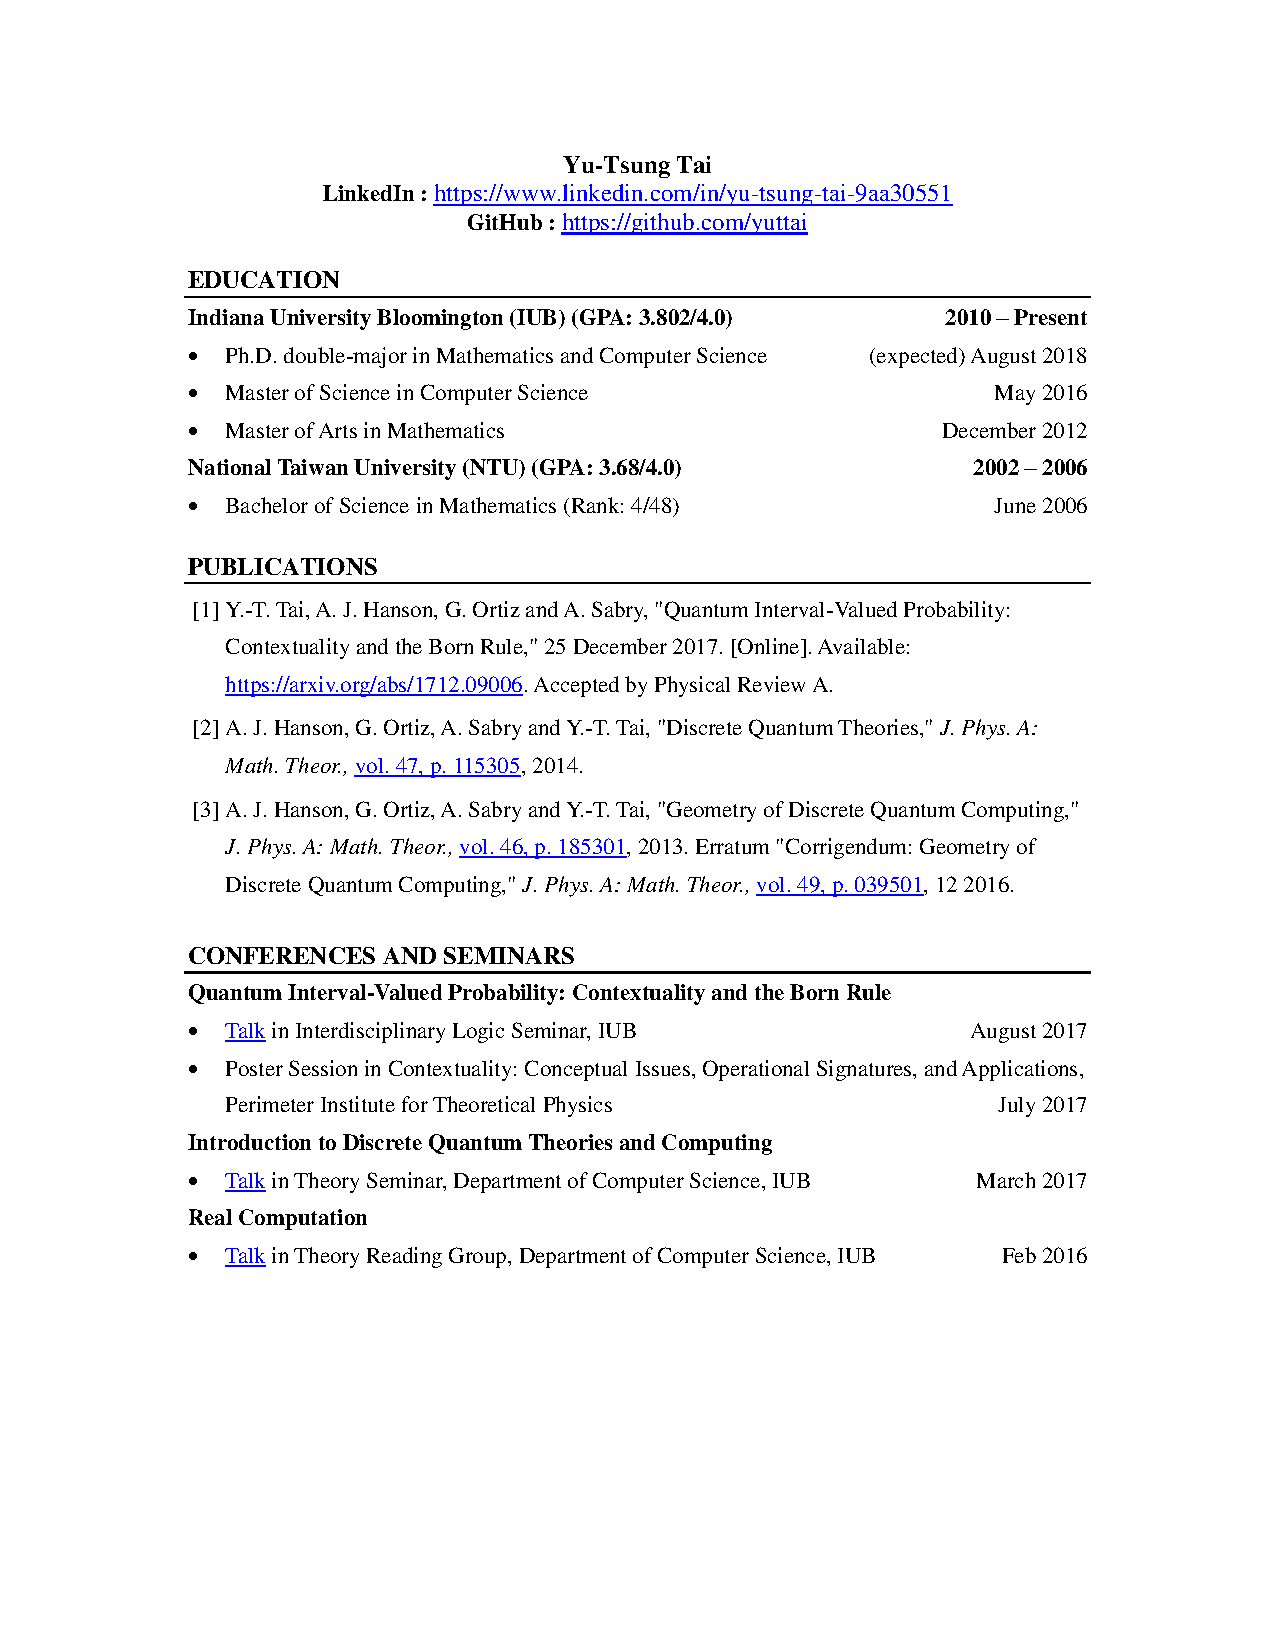
\includepdf[pages=-]{CV_thesis} 
\end{document}
